\documentclass[a4paper]{article}

%% Language and font encodings
\usepackage{abstract}
\usepackage[english]{babel}
\usepackage[utf8x]{inputenc}
\usepackage[T1]{fontenc}
\usepackage{booktabs}
\usepackage{indentfirst}
\usepackage{fancybox}
\usepackage{fancyhdr}
\usepackage{lastpage}
% \usepackage{xcolor, graphicx, float}
\usepackage{float}
\usepackage{graphicx}
\usepackage{caption}
\usepackage{subfigure}
%% Sets page size and margins
\usepackage[a4paper,top=3cm,bottom=2cm,left=3cm,right=3cm,marginparwidth=1.75cm]{geometry}

%% Useful packages
\usepackage{amsmath}
\usepackage{graphicx}
\usepackage[colorinlistoftodos]{todonotes}
\usepackage[colorlinks=true, allcolors=black]{hyperref}

\fancypagestyle{plain}%重新定义plain格式,用于summary sheet
{\fancyhf{}
\setlength{\headheight}{0pt}\setlength{\headsep}{0pt}
\setlength{\voffset}{-50pt}\setlength{\oddsidemargin}{0pt}}

\graphicspath{{pic/}}

\pagestyle{fancy} 
\lhead{Team \footnotesize{\#} 73777}
\chead{} \rhead{page\thepage\ of \pageref{LastPage}} \lfoot{}
\cfoot{\thepage}
\rfoot{}
\renewcommand{\headrulewidth}{0pt}

\makeatletter %双线页眉
\def\headrule{{\if@fancyplain\let\headrulewidth\plainheadrulewidth\fi%
\hrule\@height 1.0pt \@width\headwidth\vskip1pt%上面线为1pt粗
\hrule\@height 0.5pt\@width\headwidth  %下面0.5pt粗
\vskip-2\headrulewidth\vskip-1pt}      %两条线的距离1pt
  \vspace{6mm}}     %双线与下面正文之间的垂直间距
\makeatother


\begin{document}

\thispagestyle{empty}
\begin{minipage}{0.3\textwidth}
\begin{flushleft}
For office use only\\
   T1\ \rule{3cm}{0.5pt}\\
   T2\ \rule{3cm}{0.5pt}\\
   T3\ \rule{3cm}{0.5pt}\\
   T4\ \rule{3cm}{0.5pt}\\
\end{flushleft}
\end{minipage}\hspace{\fill}
\begin{minipage}{0.3\textwidth}
\centering
Team Control Number\\[5pt]
\fontsize{36pt}{\baselineskip}\selectfont  \textbf{73777} \normalsize\\[10pt]
Problem Chosen\\[5pt]
\fontsize{18pt}{\baselineskip}\selectfont \textbf{C}\normalsize\\
\end{minipage}\hfill
\begin{minipage}{0.35\textwidth}
\begin{flushright}
\shortstack[l]{
For office use only\\
   F1\ \rule{3cm}{0.5pt}\\
   F2\ \rule{3cm}{0.5pt}\\
   F3\ \rule{3cm}{0.5pt}\\
   F4\ \rule{3cm}{0.5pt}}
\end{flushright}
\end{minipage}\vspace*{10pt}
\rule{\textwidth}{0.5pt}

\begin{center}
  \textbf{2018}
\end{center}
\begin{center}
  \textbf{MCM/ICM}
\end{center}
\begin{center}
  \textbf{Summary Sheet}
\end{center}

%\enlargethispage
{\begin{center}\Large \textbf{Energy System Assessment and Interstate Contract Model in Four U.S. States}\end{center}}

First of all, in this paper, the data of four states are processed separately. The features of each aspect are selected and the energy profiles of the four states are described in detail.


Secondly, this paper chooses some clean energy features, uses the illustrated method to explain the consumption of clean energy and each sector's expenditure, and chooses 8 + 5 different categories of features related to clean energy, through PCA analysis Method to describe the consumption and expenditure of various states, including nuclear power, geothermal, renewable energy and other types of clean energy.

After that, this paper chooses several clean energy features, including the energy consumption, the average energy price, the output of clean energy, the expenditures of various sector, and the TOPSIS tool to get the annual comprehensive energy evaluation index of four states. Through the comprehensive index, Throughout the state's clean energy use over the years to conduct an analysis of the four states in different years to use different levels of clean energy index. At the same time, the composite features also reflect the clean energy consumption of each state in each year, the expenditures of various sector, the output and consumption of different kinds of energy sources.

Then, this paper constructs a multiple regression model, selects six factors that have influence on energy and closely related to each state, analyzes the weight of six features in each state, and shows the influence factors by the positive and negative weight and size The way and extent of the impact on the importance of energy eventually led to the evaluation of the profile of the states in 2009. The result is CA(California)>TX(Texas)>AZ(Arizona)>NM(New Mexico State), and a detailed explanation of the similarities and differences between the states.

In addition, this paper also uses a gray model to predict the state's clean energy index in the next 2025 and 2050 by expanding the five-year clean energy comprehensive index of the four states, and test the forecast results It shows that the model has high accuracy and the data is credible. The final prediction shows that AZ> CA> NM> TX, AZ has great potential for development.

After defining the present, future state of energy in each state, this article gives comments on the signing of interstate contracts. According to the results of the data analysis and the differences among the four states, each state should be given a suitable future energy goal respectively, and in order to achieve the goal, it should give pertinent suggestions on corresponding actions that the states should take.

Finally, although the model constructed in this article is theoretically strong, innovative , credible, and  of practical significance, there are still some shortages in the process of building and analyzing the model. Due to the fact that further breakthroughs are needed in the selection of data-oriented features.


{\bfseries keywords:} PCA, energy planning, energy contract model, gray prediction, topsis method

\newpage
\thispagestyle{empty}
\setcounter{page}{0}
{\begin{center}\Large \textbf{Energy System Assessment and Interstate Contract Model in Four U.S. States}\end{center}}
\tableofcontents                                                  
\newpage 

\section{Problem restatement}

We will clarify the ideas and context below based on the background of the subject, data, repeat the problem. Then, we will follow the steps in order to answer the question.

\begin{itemize}

\item 1. Graphs and brief descriptions can be regarded as an overview of each state's energy.

\item 2. Describe the historical development of clean energy in all states, and use a comprehensive evaluation index of clean energy to summarize the development of clean energy in all states by year.

\item 3. Then, based on the above results, we analyzed the differences among the various states and the differences between states.

\item 4. According to the comprehensive evaluation index of clean energy, we can get the ranking of clean energy use by each state in 2009. And predict the state's comprehensive assessment of clean energy in 2025 and 2050.

\item 5. Based on the above analysis and findings, we give the best standards of energy use as a target and find the problems in each state, and give some strategies to solve the problems so that the states can approach the best energy sources Usage.

\end{itemize}

And some features in this paper was calculated by 605 variables, the specific steps are complex but using traditional statistical method. So we avoid giving too much unnecessary details here.

\section{Energy profile}

\subsection{Regular of the data}

Among the energy consumption information of the four states, data extraction and statistics make it easy to find that there are 318 features in 1960-1969, 576 features in 1970-1976, 578 features in 1977-1979, 583 features as the following table. In other words, not all have values, some of the values are vacant.

\begin{table}[!htbp]
\centering
\begin{tabular}{cc}
\toprule
Years & Variables numbers provided\\
\midrule
1960-1969 & 318\\
1970-1976 & 576\\
1977-1979 & 578\\
1980-2009 & 583\\
\bottomrule
\end{tabular}
\caption{Structure of source data}\label{tab:aStrangeTable}
\end{table}

According to the attribute characteristics of datasets, we classify them according to the three dimensions of different sectors, different numerical units and different attributes of resources. We think that all the data in the dataset can be divided into the following seven categories: Gas energy consumption, Polluted energy consumption, Clean energy consumption, Solid energy consumption, Liquid energy consumption, Electricity energy consumption, the sum of all the expenditure costs of various sectors in terms of energy consumption.

It should be noted that, in the data processing, we will think hydro power, nuclear power, fuel ethanol and ethanol, natural gas, liquefied petroleum gas, geothermal, etc. as a clean energy. As the cleanliness and economy of energy are more important for energy choices and planning, we focus on three sources of polluted energy, clean energy, and total expenditure on resources by sectors aspect.

\subsection{Data preprocessing}
\subsubsection{Data screening and feature extraction(18 features)}

\begin{table}[H]
\centering
\begin{tabular}{cc}
\midrule
All polluted energy consumption& All clean energy consumption\\
Liquid polluted energy consumption& Liquid clean energy consumption\\
Solid polluted energy consumption& Solid clean energy consumption\\
Electricity clean energy consumption& Gaseous clean energy consumption\\
Polluted energy  expenditures in the commercial sector& Clean energy  expenditures in the commercial sector \\
Polluted energy  expenditures in the industrial sector &  Clean energy  expenditures in the industrial  sector\\
Polluted energy  expenditures in the electric power sector & Clean energy  expenditures in the electric power sector \\
Polluted energy  expenditures in the residential sector & Clean energy  expenditures in the residential sector \\
Polluted energy  expenditures in the transportation sector&Clean energy  expenditures in the transportation sector\\
\bottomrule
\end{tabular}
\caption{Available features}\label{tab:aStrangeTable}
\end{table}

\subsection{Compress characteristics by principal component analysis(PCA)}

The first eight features can be compressed into two features: All polluted energy consumption and all clean energy consumption.

Here is the processing method\cite{pca}:

Standardized collection of original index data.
8 dimensional random vector $x = (x_1, x_2, ..., x_8)^{T}$, 50 samples $x_i = (x_{i1}, x_{i2}, ...,x_{i8}), i=1,2,..,50$. Then structural sample array,make the following standardized changes to the sample array:\[
Z_{ij}=\frac{X_{ij}-\bar{x_j}}{s_j},\quad i = 1, 2,..,50 \quad j = 1, 2, ..,8
\]

In which $\bar{x_j}=\frac{\sum_{i=0}^{n}{x_ij}}{n}$, $s^{2}_{j}=\frac{\sum_{i=1}^{n}{x_{ij}-\bar{x_j}}^{2}}{n-1}$ , get the standardized array Z.

Solving correlation coefficient matrix for the standardized array Z.

\[R = [r_{ij}]_{p} = \frac{Z^{T}Z}{n-1},\quad i,j=1,2,..,p\]

Solving the characteristic equation of sample correlation matrix R $|R - \lambda I_p| = 0$, to get p characteristic roots and to determine principal component.
According to $\frac{\sum_{j=1}^{n}{\lambda_{j}}}{\sum_{j=1}^{p}{\lambda_{j}}} \geq 0.85$, determine the m value to make the information utilization more than 85%.

For each $\lambda_{i}, j = 1,2,...,m$, solve equation set to get the unit eigenvector $b_{j}^{o}$

Converting the normalized index variables to the main component.

\[U_{ij} = z_{i}^{T}b_{i}^{o},\quad j = 1,2,...,8\]

$U_1$ is called the first principal component, $U_2$ is called the second principal component. 

Therefore, we can compress the clean energy (energy + solid + liquid + gas + electric) into a series of characteristics. The polluted energy (energy + solid + liquid) is compressed into a series of characteristics. That is, the two column now.


\subsection{Data visualization}

By PCA analysis, we now have 12 features for every year of each state. According to these features, we can draw two charts for each states. The two charts show the consumption of two kinds of energy and the expenditures of two kinds of energy in the five sectors.

\begin{figure}[H]
\begin{minipage}[t]{0.5\linewidth}
\centering
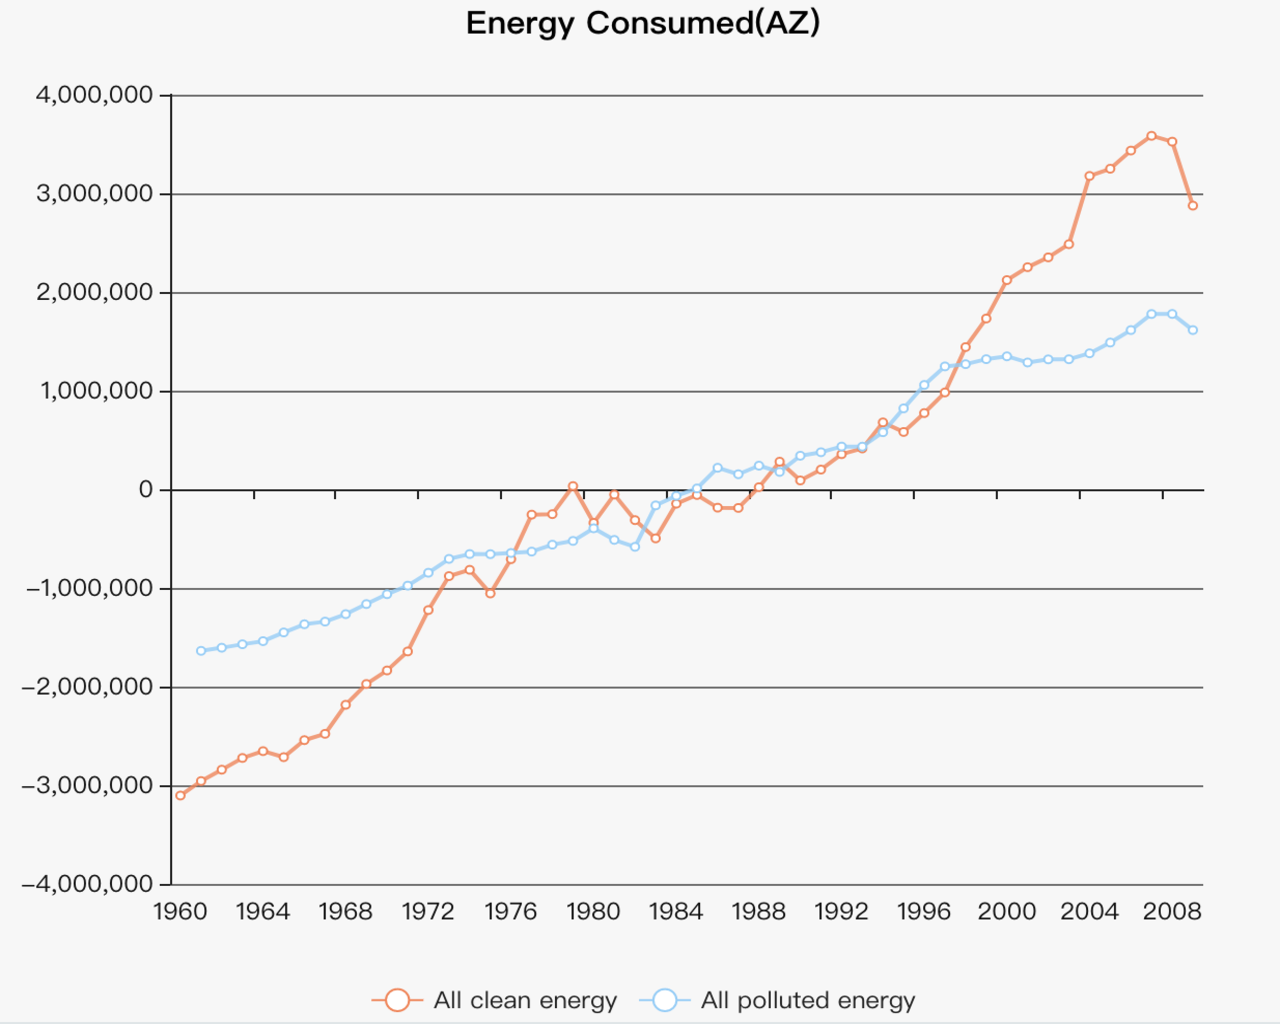
\includegraphics[width=2.2in]{./Energy-Com-AZ_gaitubao_com_1280x1024.png}
\label{fig:side:a}
\end{minipage}%
\begin{minipage}[t]{0.5\linewidth}
\centering
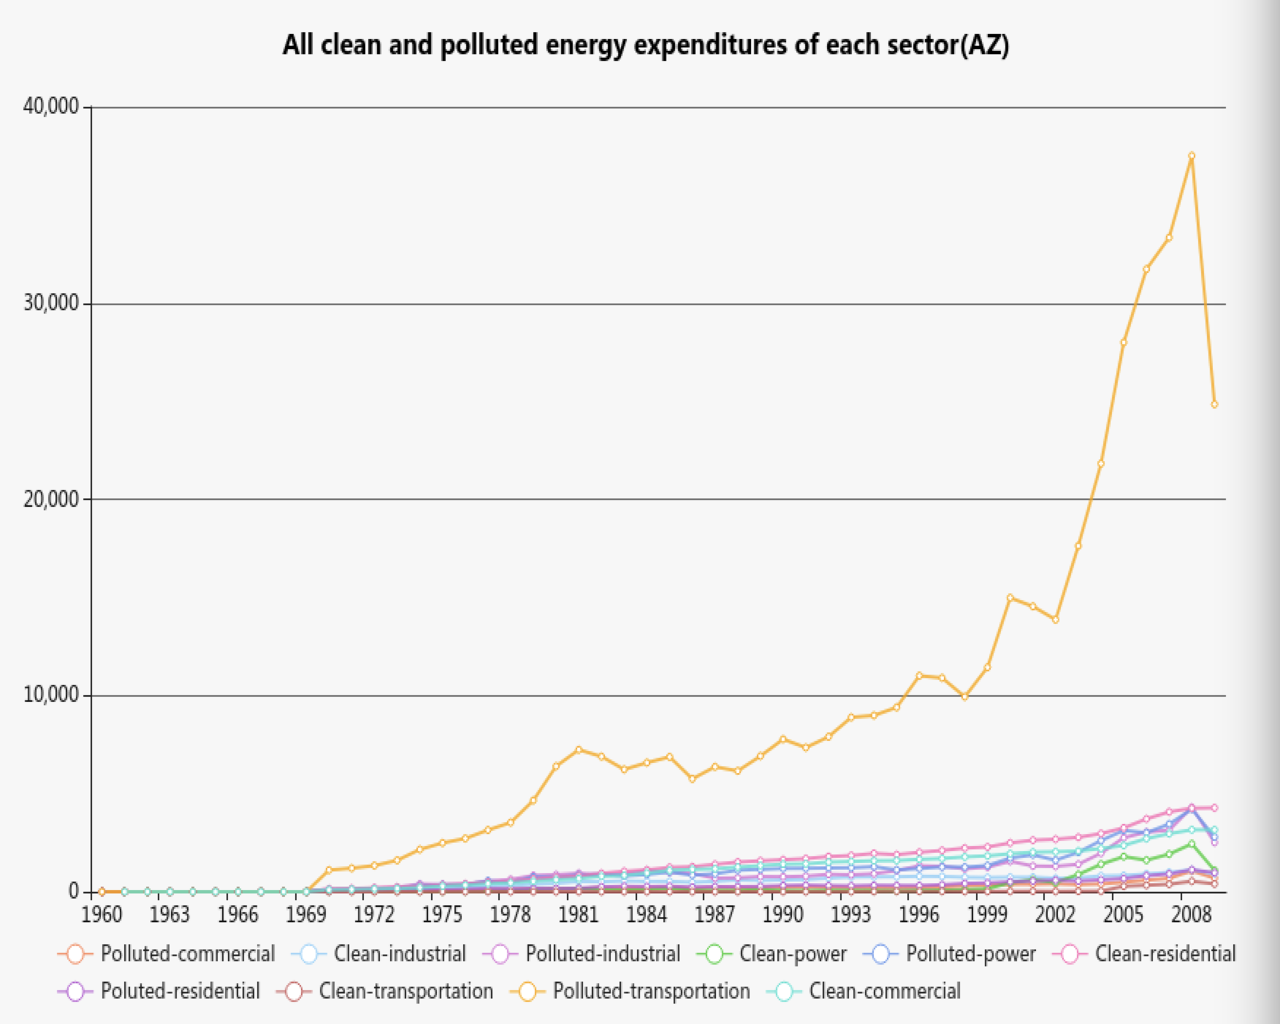
\includegraphics[width=2.2in]{./Sector-AZ_gaitubao_com_1280x1024.png}
\label{fig:side:b}
\end{minipage}
\caption{Energy consumption and expenditures(AZ)}
\end{figure}

\begin{enumerate}
\item The polluted energy consumed by AZ state was more stable, showing a trend of increasing year by year. The growth of clean energy consumption from 1978 to 1988 did not increase in other years, presuming that the relevant policies may have changed.

\item In terms of energy expenditures in each sectors, the most was still polluted energy expenditure in the transportation sector. More considerable, clean energy expenditure in the residential sector accounted for second,  indicating that the residential people are generally aware of the use of clean energy.
\end{enumerate}

\begin{figure}[H]
\begin{minipage}[t]{0.5\linewidth}
\centering
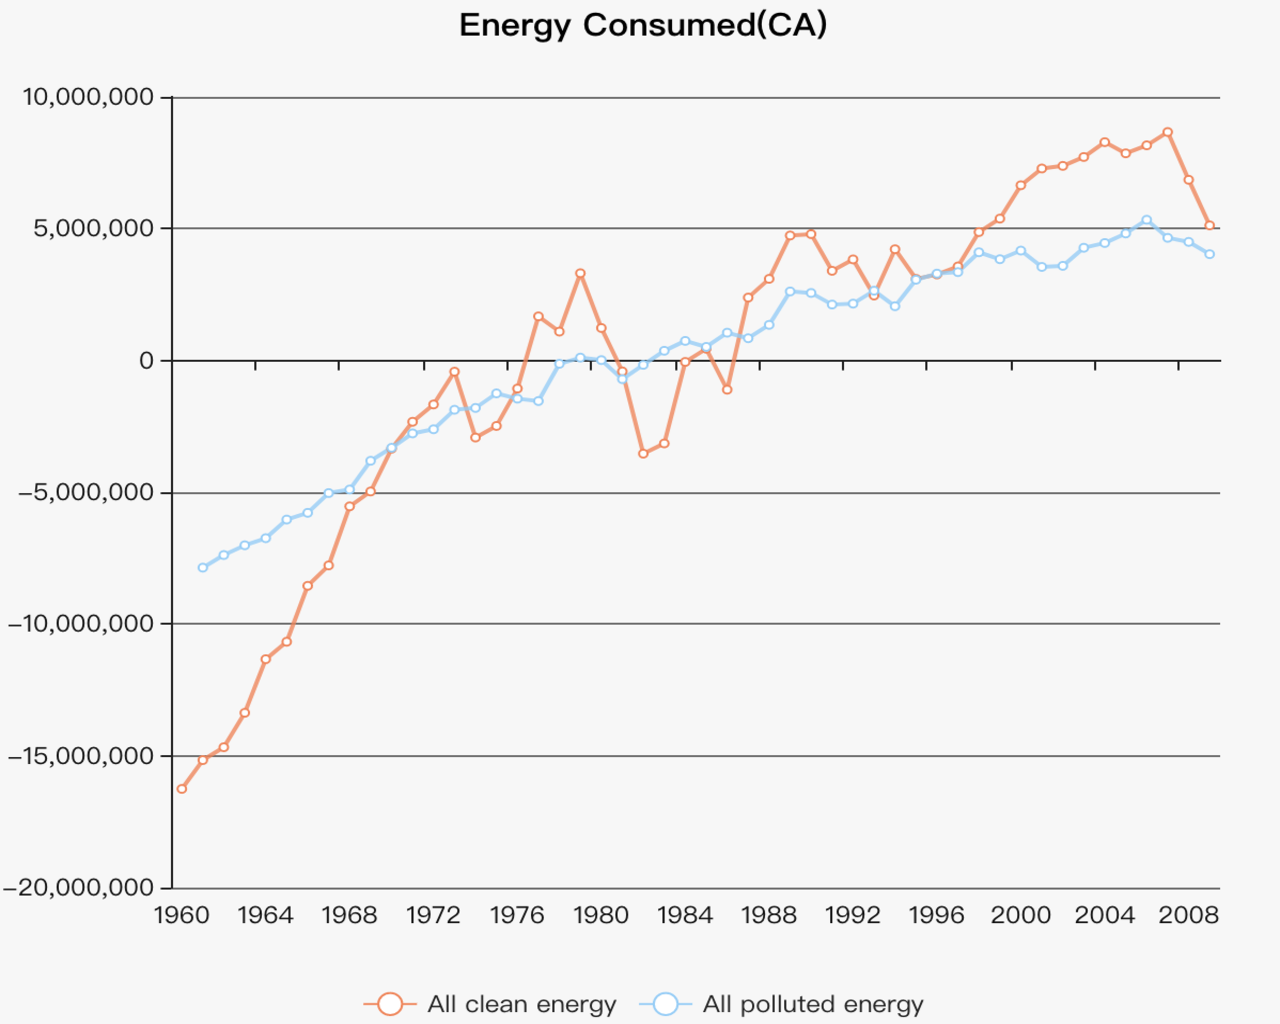
\includegraphics[width=2.2in]{./Energy-Com-CA_gaitubao_com_1280x1024.png}
\label{fig:side:a}
\end{minipage}%
\begin{minipage}[t]{0.5\linewidth}
\centering
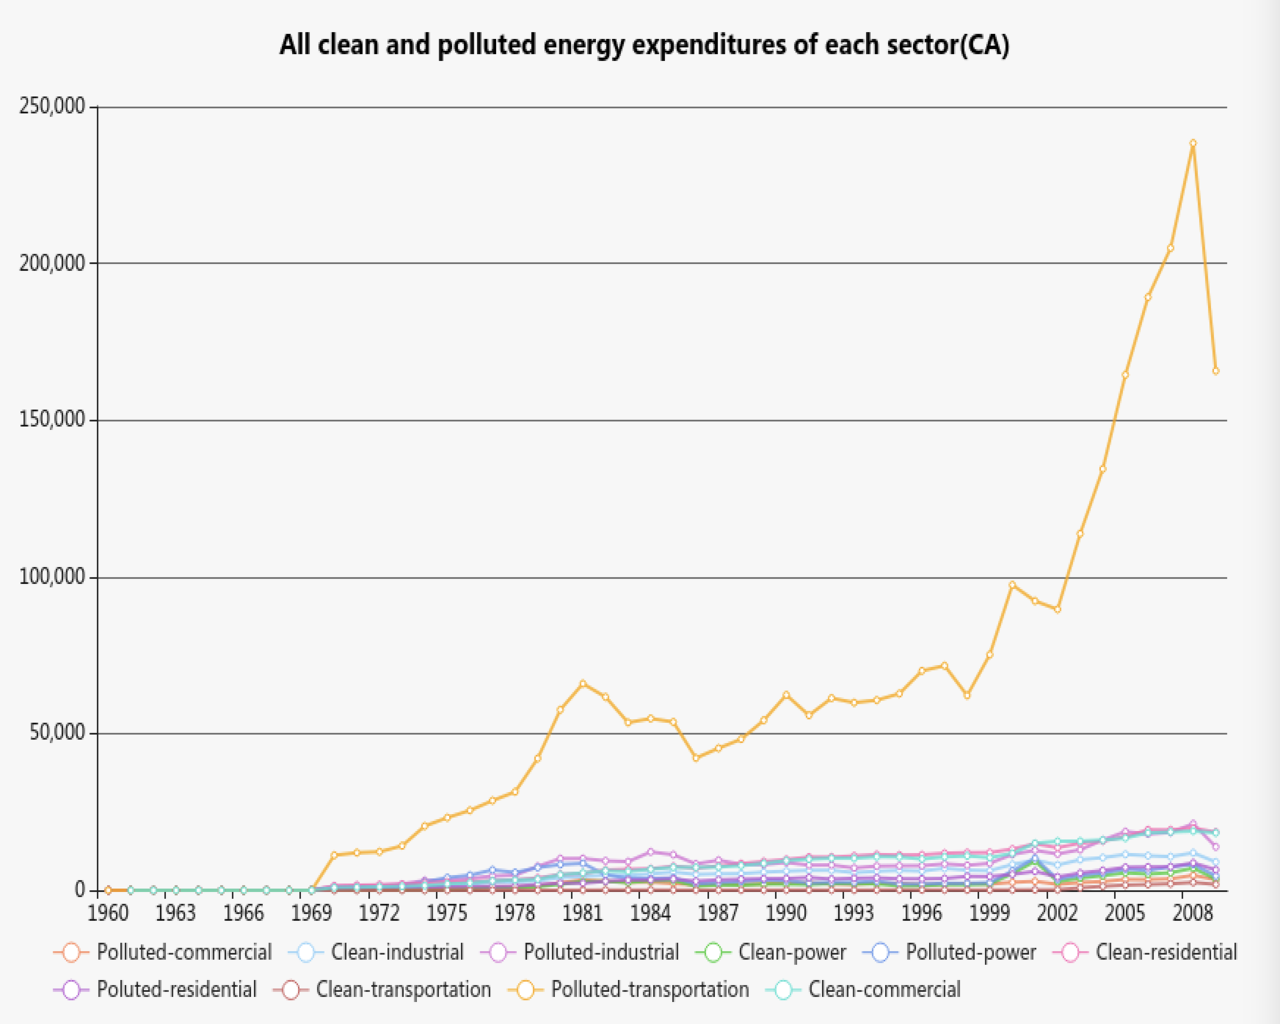
\includegraphics[width=2.2in]{./Sector-CA_gaitubao_com_1280x1024.png}
\label{fig:side:b}
\end{minipage}
\caption{Energy consumption and expenditures(CA)}
\end{figure}

\begin{enumerate}
\item The polluted energy consumed by CA state was more stable, showing a trend of increasing year by year.There was a significant fluctuation in clean energy consumption from 1978 to 1988, which was presumed to be a change in the relevant policies. It was likely that the authorities focused on economic development.

\item In terms of energy expenditures in each sectors, the most was still polluted energy expenditure in the transportation sector.Other sectors spent more on polluted energy than clean energy, showing that the state of CA was still based on the industry of polluting energy, so the economy was developing rapidly, but was still needs to pay attention to environmental problems and promoted the reform of industrial structure.
\end{enumerate}


\begin{figure}[H]
\begin{minipage}[t]{0.5\linewidth}
\centering
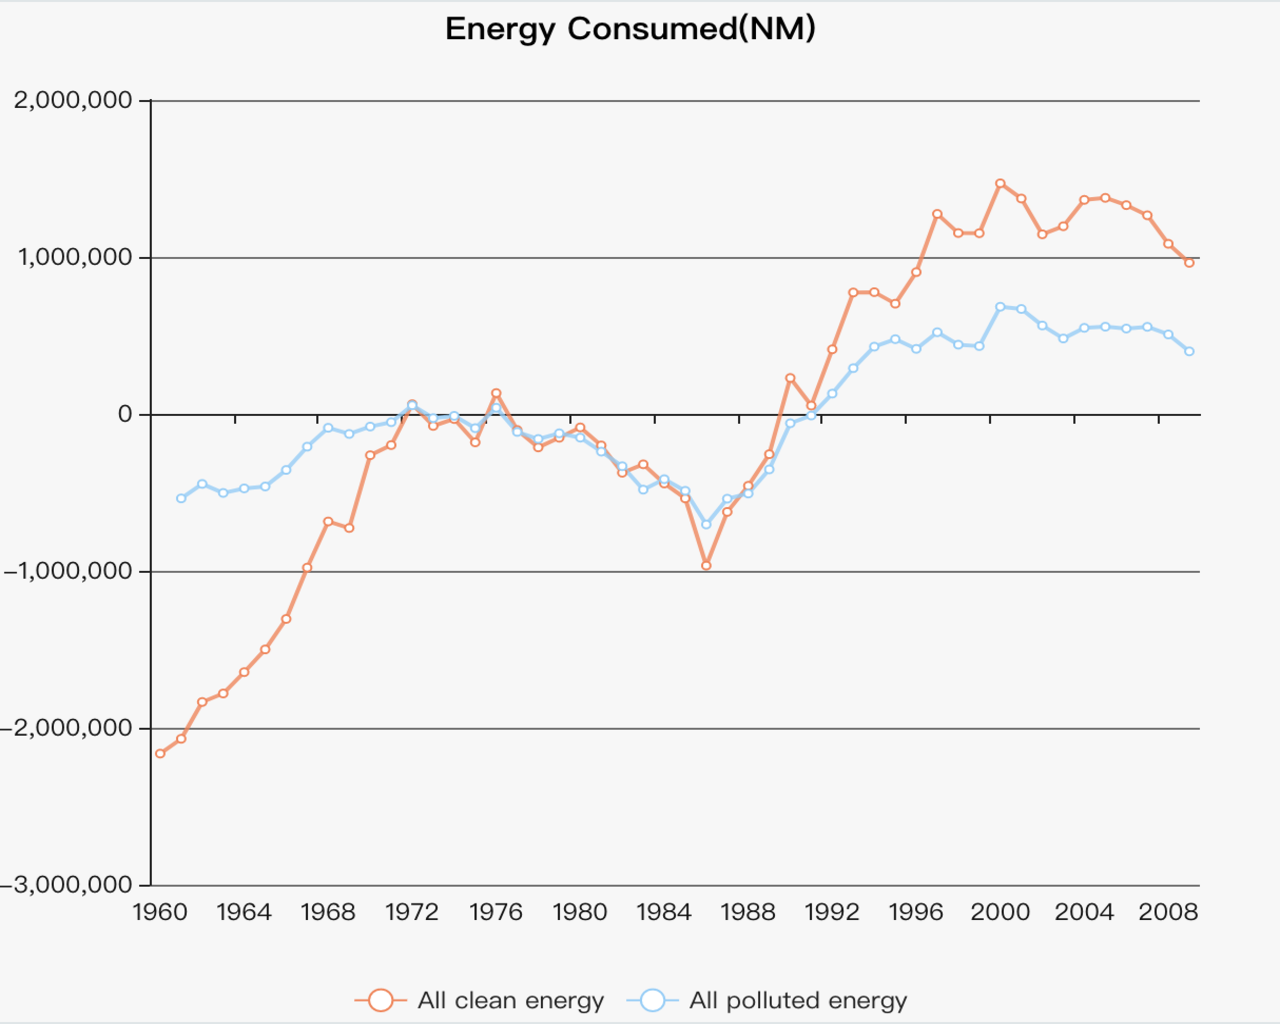
\includegraphics[width=2.2in]{./Energy-Com-NM_gaitubao_com_1280x1024.png}
\label{fig:side:a}
\end{minipage}%
\begin{minipage}[t]{0.5\linewidth}
\centering
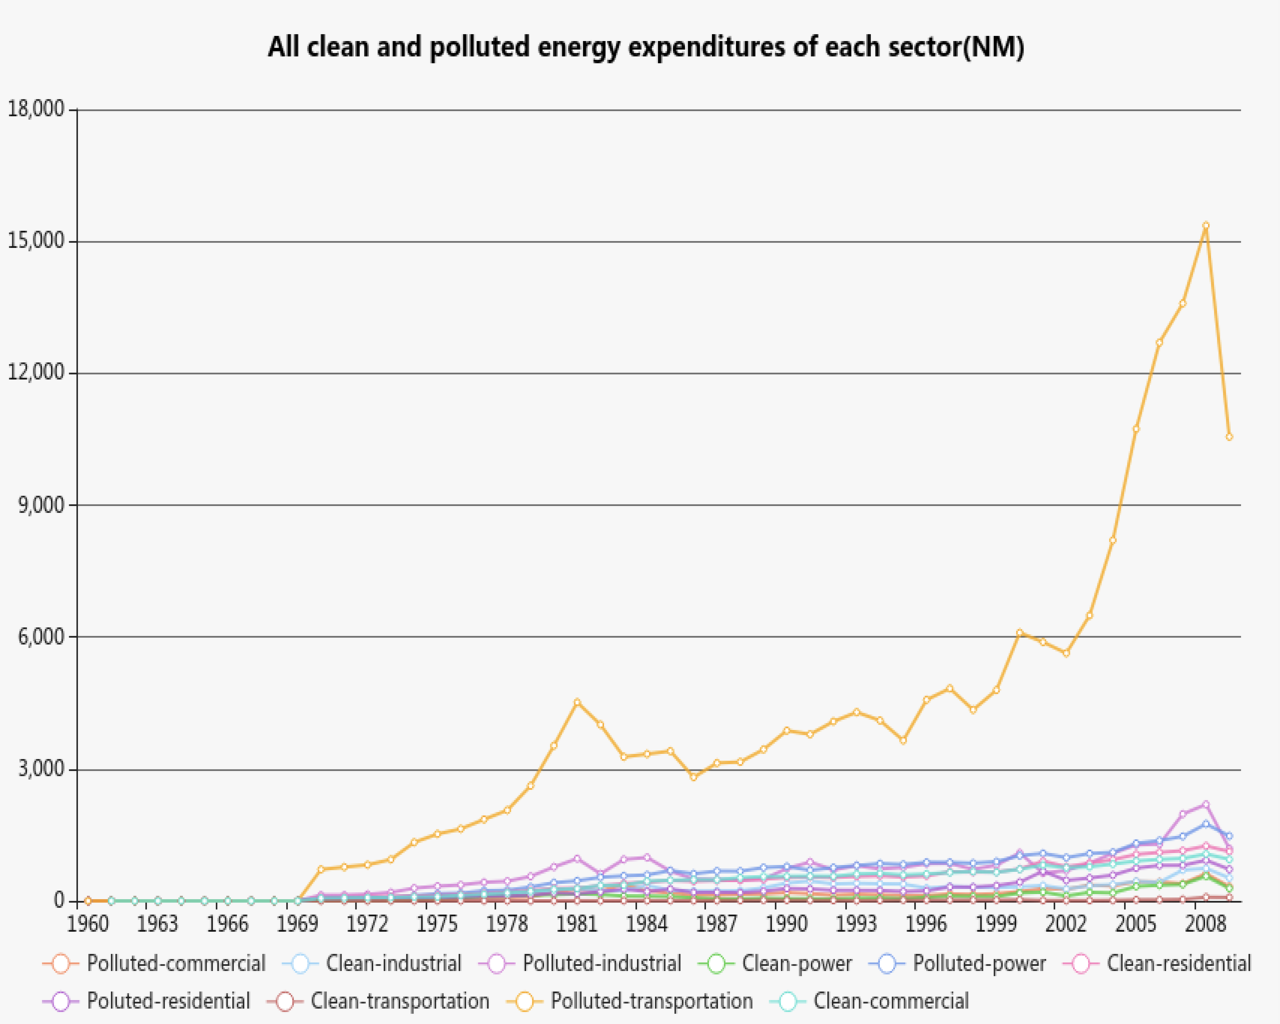
\includegraphics[width=2.2in]{./Sector-NM_gaitubao_com_1280x1024.png}
\label{fig:side:b}
\end{minipage}
\caption{Energy consumption and expenditures(NM)}
\end{figure}

\begin{enumerate}
\item The energy consumption and clean energy consumption in NM state fluctuated significantly from 1976 to 1996, and reached a trough in about 1986, indicating that the energy consumption of NM state in 1980s was too low. And the growth was not high after both, presumably related to major policy issues, and because of the regional inhabitable climate that lead to slower energy development.

\item In terms of energy expenditures in each sectors, the most was still polluted energy  expenditure in the transportation sector, followed by  polluted energy expenditure in the industrial sector,  indicating that because of its rich energy,the NM state had more industrial development, so the energy structure was still the majority of the polluted energy.
\end{enumerate}



\begin{figure}[H]
\begin{minipage}[t]{0.5\linewidth}
\centering
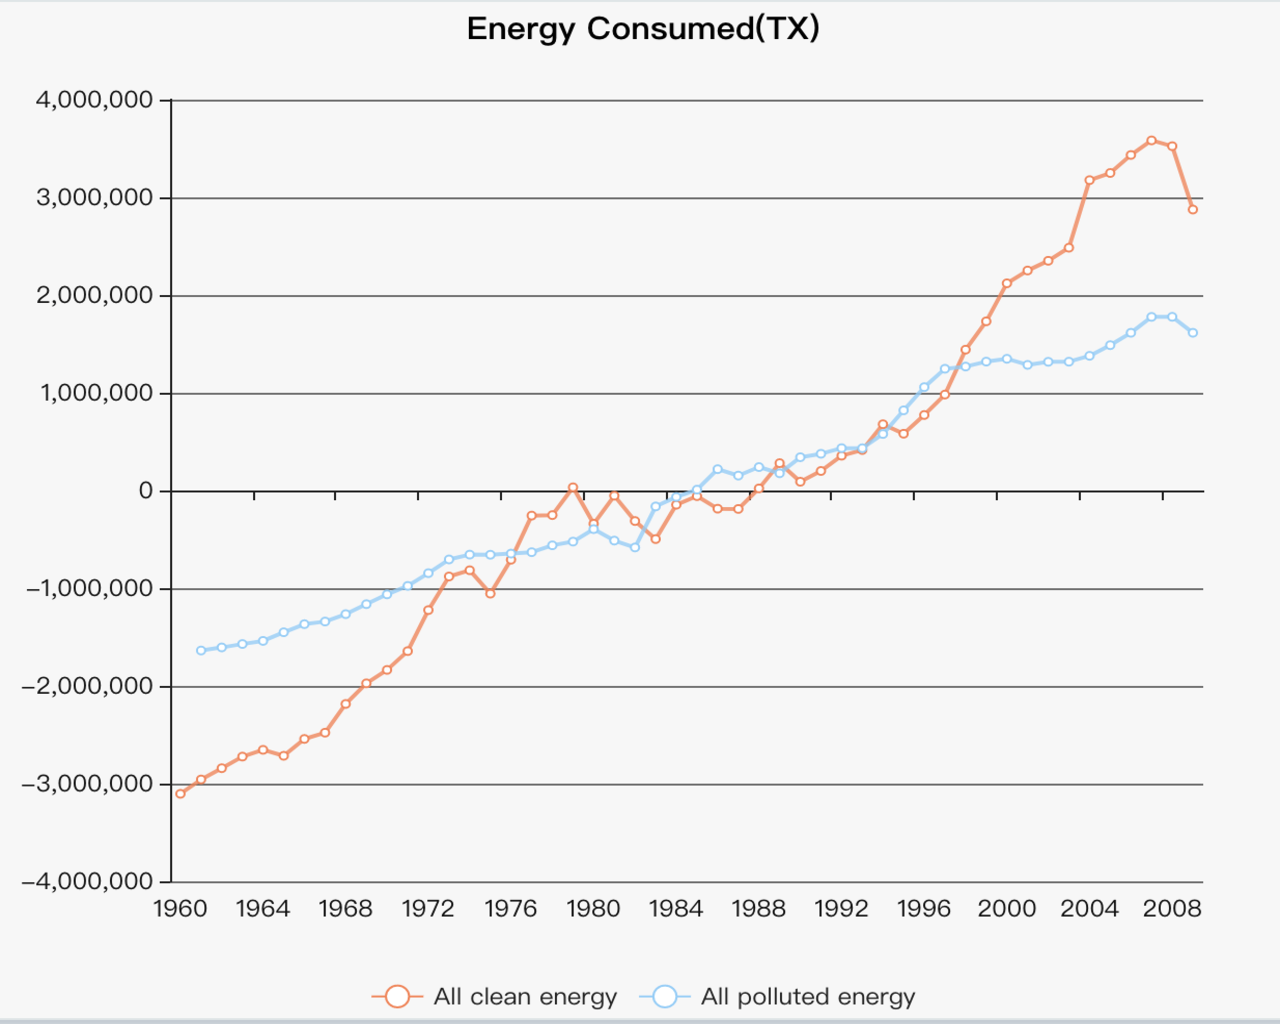
\includegraphics[width=2.2in]{./Energy-Com-TX_gaitubao_com_1280x1024.png}
\label{fig:side:a}
\end{minipage}%
\begin{minipage}[t]{0.5\linewidth}
\centering
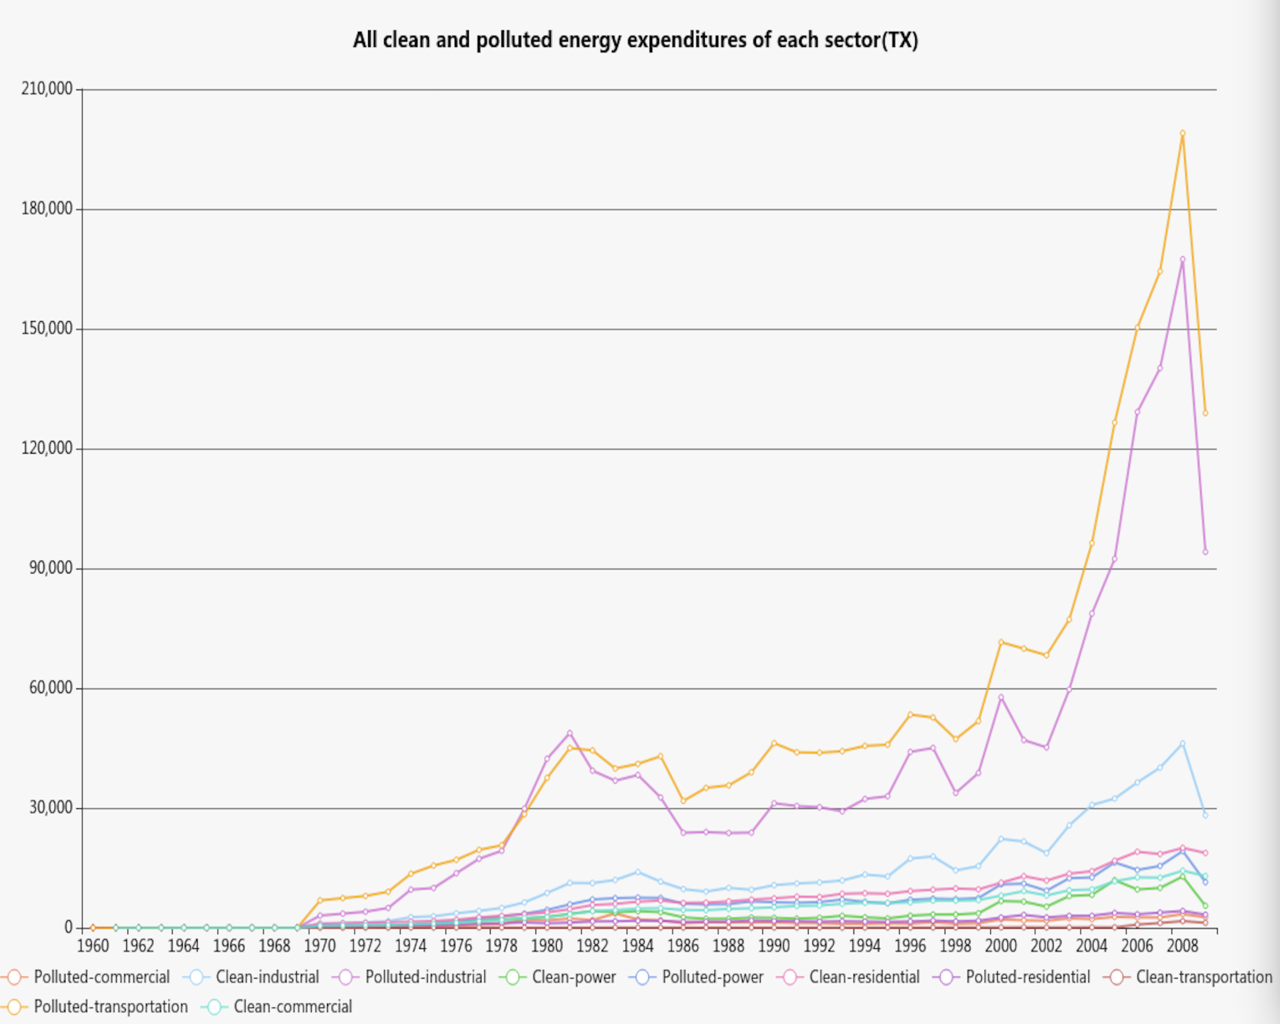
\includegraphics[width=2.2in]{./Sector-TX_gaitubao_com_1280x1024.png}
\label{fig:side:b}
\end{minipage}
\caption{Energy consumption and expenditures(TX)}
\end{figure}

\begin{enumerate}
\item The consumption of polluted energy in TX state was relatively slow, but the growth rate was slow. Clean energy consumption had fluctuated from 1976 to 1988, and the frequency of volatility was not high, but it was growing fast after about 1988. It showed that energy consumption in TX state was more stable, and the speed of clean energy consumption was quicker.

\item In terms of energy expenditures in each sectors,  polluted energy expenditure in the transportation sector and residential sector  were the biggest , and there was little difference between them. Moreover, polluted energy expenditure in the electricity power sector was also large. It might be related to more population and geographical environment, and it was located in the temperate subtropical climate zone, which might be related to excessive use of air conditioning.
\end{enumerate}



\subsection{General profile of four states}

Based on the above eight figures, we can see that, with the growth of the year, the four provinces are developing faster, and the industrialization and urbanization process is accelerating. The demand for energy is increasing, and the consumption of clean energy and polluted energy is increasing. 

Before the mid 90s, the energy consumption of the four states was dominated by non clean energy, but after the middle of 90s, the energy consumption structure was transformed. The consumption of clean energy in four states generally exceeded the consumption of non clean energy. 

In terms of clean energy and polluted energy expenditures in different sectors of the four states, the  polluted energy expenditure in  transportation sector is generally higher than that in other sectors. But around 2007, all of the energy expenditures, especially on polluted energy expenditure in the commercial sector, had fallen.\cite{consumption}

In general, we can draw several characteristics of the energy profile of these four states:

\begin{enumerate}
\item Energy demand is growing over time.
\item The supply capacity has been significantly improved.
\item The consumption structure has been optimized, but it is not thorough enough.
\item The level of science and technology has rapidly increased, which can be seen from the decline in energy consumption and expenditure
\end{enumerate}

\section{Evolution of clean and reliable energy}

How to describe the usage of clean and reliable energy in a year? We think it can be concluded in four different aspects: consumption, the consumption of various types of clean and reliable energy, expenditures of each sector and the production of clean energy.

\subsection{Features selection}

We choose the following 22 features to find out general characteristics:

\begin{table}[H]
\centering
\begin{tabular}{cc}
\midrule
Clean normal energy consumption & Clean fluid energy consumption\\
Clean gas energy consumption & Clean electric energy consumption\\
Clean energy  expenditures in the commercial sector& Clean energy expenditures in the industrial sector \\
Clean energy expenditures in the electric sector&Clean energy expenditures in the residential sector\\
Clean energy expenditures in the transportation power sector & Biomass total consumption \\
Fuel ethanol consumption & Electricity consumption \\
Geothermal energy consumption & Natural gas consumption \\
Renewable energy consumption & Supplemental gaseous fuels consumption\\
Photovoltaic and solar thermal energy consumption & Geothermal production \\
Hydroelectricity production & Nuclear power production \\
Renewable energy production &wind energy\\
\bottomrule
\end{tabular}
\caption{Clean and reliable energy relevant features}\label{tab:aStrangeTable}
\end{table}

\subsection{Data visualization}

In order to show the characteristics of the usage of clean energy, we draw 3 statistical charts for each state using traditional statistical methods, including consumption, expenditures and types.

\begin{figure}[H]
\begin{minipage}[t]{0.5\linewidth}
\centering
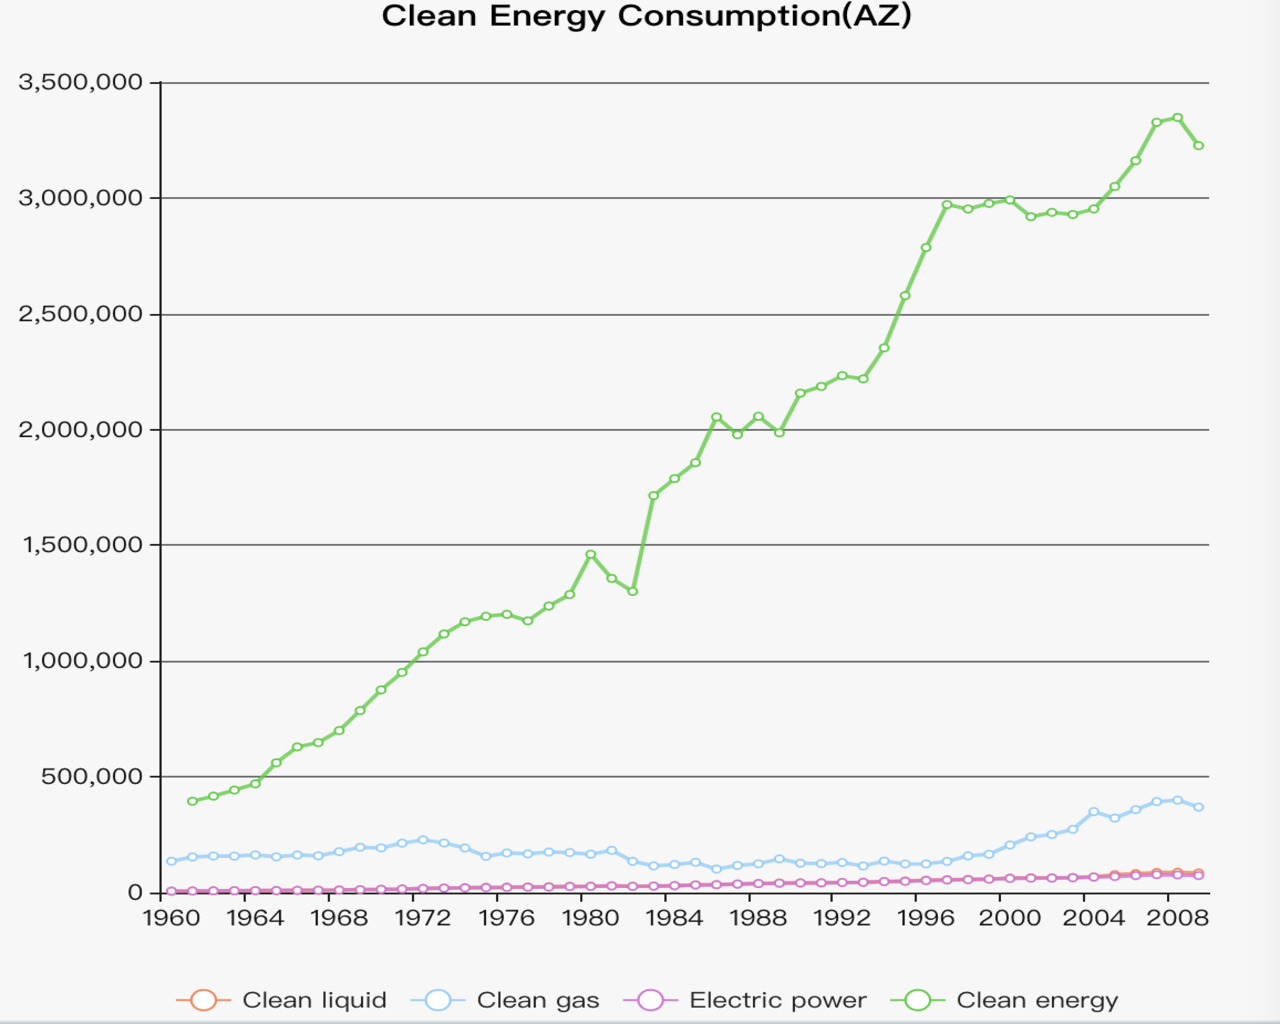
\includegraphics[width=2.2in]{./01_gaitubao_com_1280x1024.png}
\label{fig:side:a}
\end{minipage}%
\begin{minipage}[t]{0.5\linewidth}
\centering
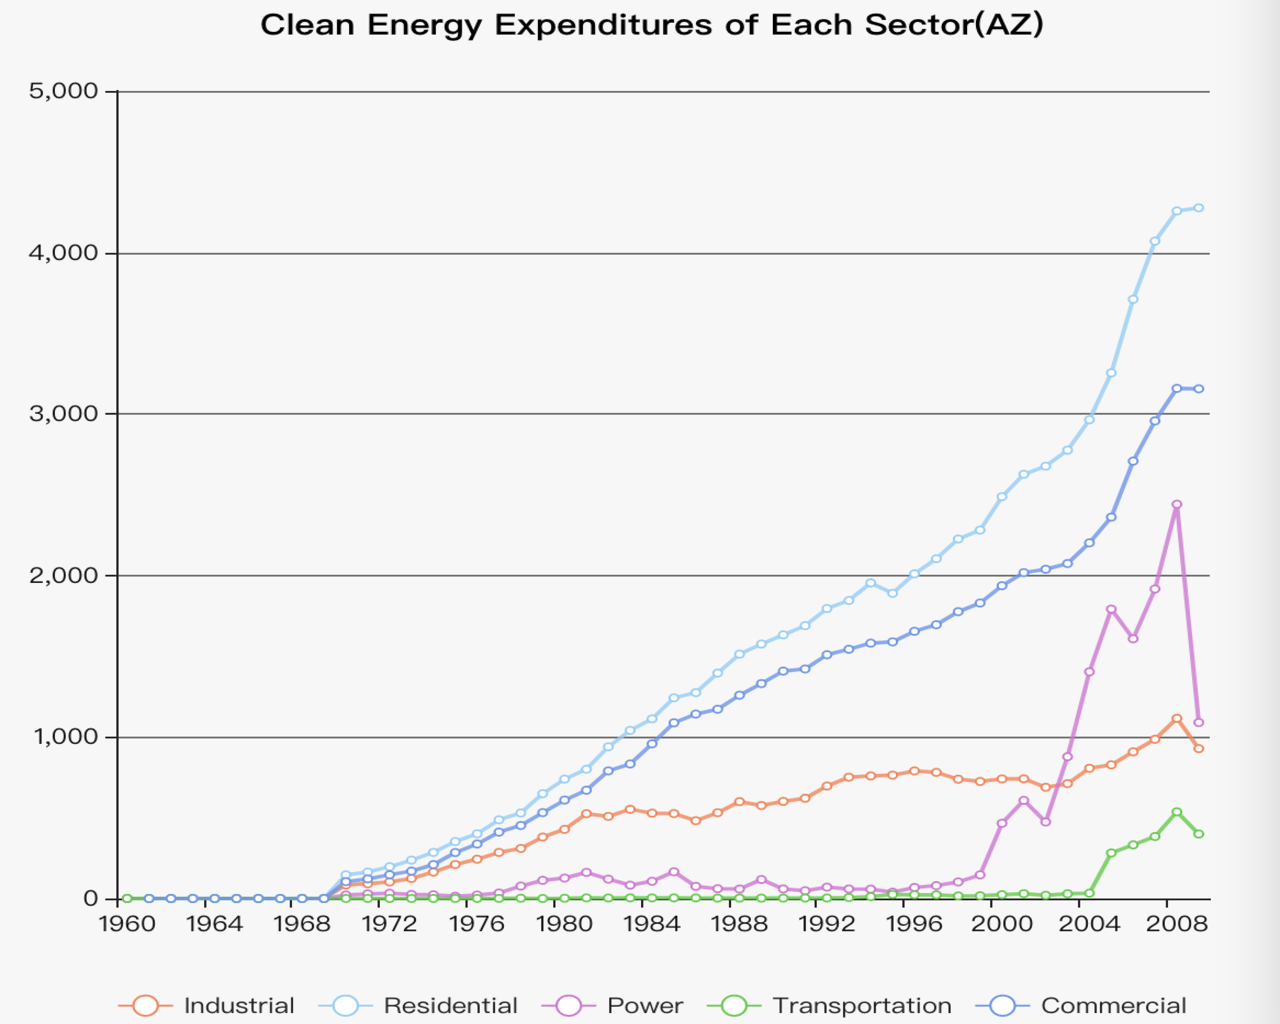
\includegraphics[width=2.2in]{./03_gaitubao_com_1280x1024.png}
\label{fig:side:b}
\end{minipage}
\end{figure}

\begin{figure}[H]
	\begin{center}
		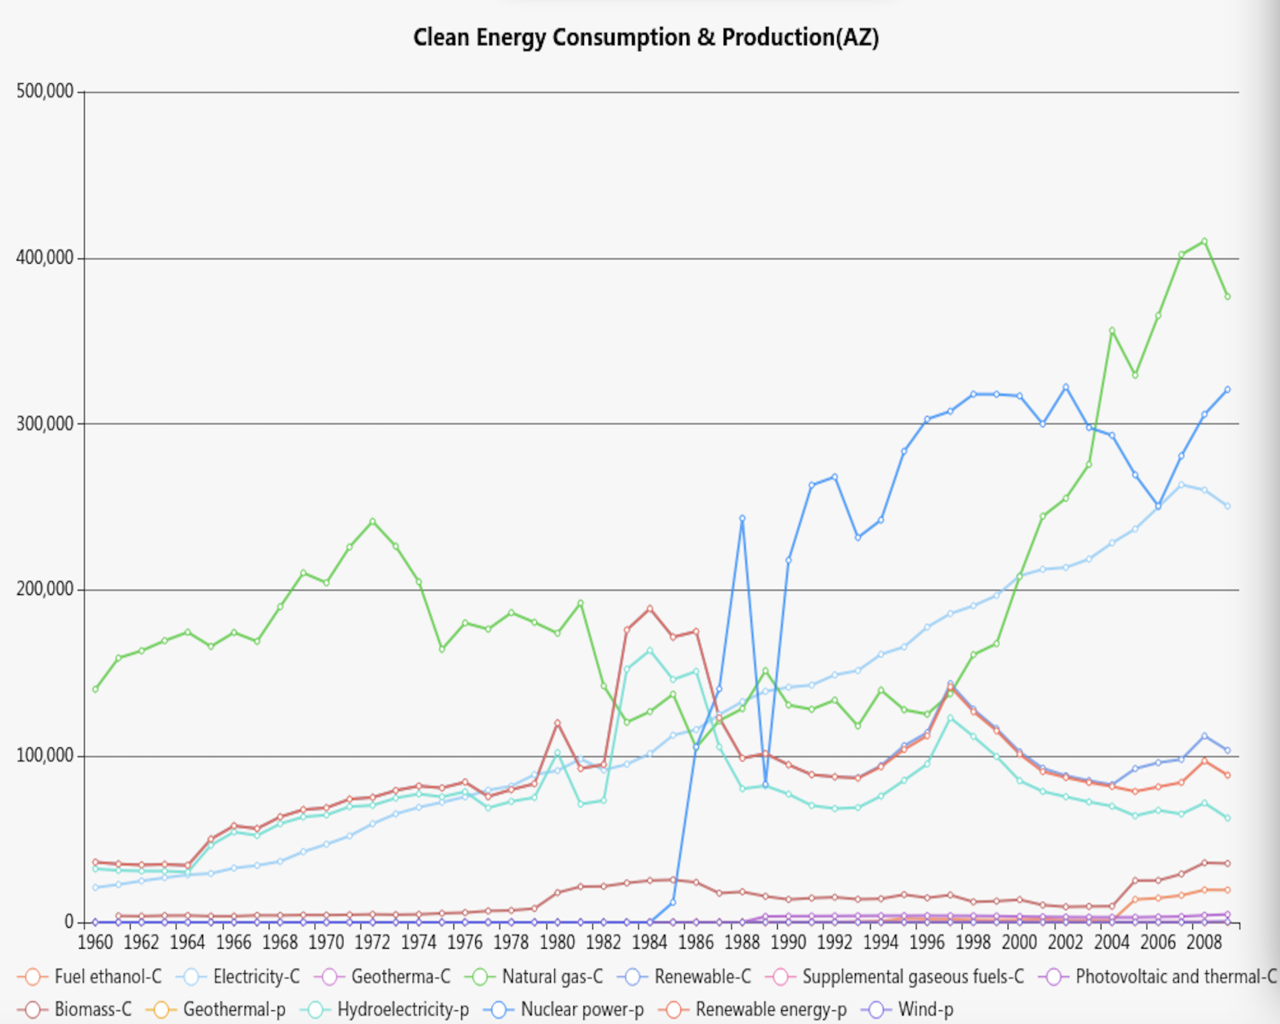
\includegraphics[width=0.5\linewidth]{2018021200471898854AZZZ.png}
		\caption{Evolution of clean and reliable energy(AZ)}
		\label{Fig:1}
	\end{center}
	\vspace{-0.5em}
\end{figure}

\begin{enumerate}
\item The clean energy consumption in AZ state has been fluctuating in the period of 1960-2009. The consumption of natural gas is generally higher than that of electric power.

\item In terms of the clean energy expenditures in each sectors of AZ state,the residential sector was the largest ,followed by the commercial sector , and the two increased significantly around 2002. And expenditure in the electric power sector has also increased significantly after 2002, and that in the transportation sector has also increased significantly after 2004. Expenditure in the industrial sector is rising relatively smoothly.

\item In terms of clean energy consumption or production of AZ state,the consumption of natural gas and the consumption of electricity account for the most. Nuclear power generation has developed rapidly since 1984, and has gone through the trough of 1988 to become the main mode of production, and there is an upward trend. Other energy consumption and output trends are relatively stable, but all fluctuate in 1980-1988. It is worth mentioning that the state's wind power consumption has been in the doldrums.

\end{enumerate}



\begin{figure}[H]
\begin{minipage}[t]{0.5\linewidth}
\centering
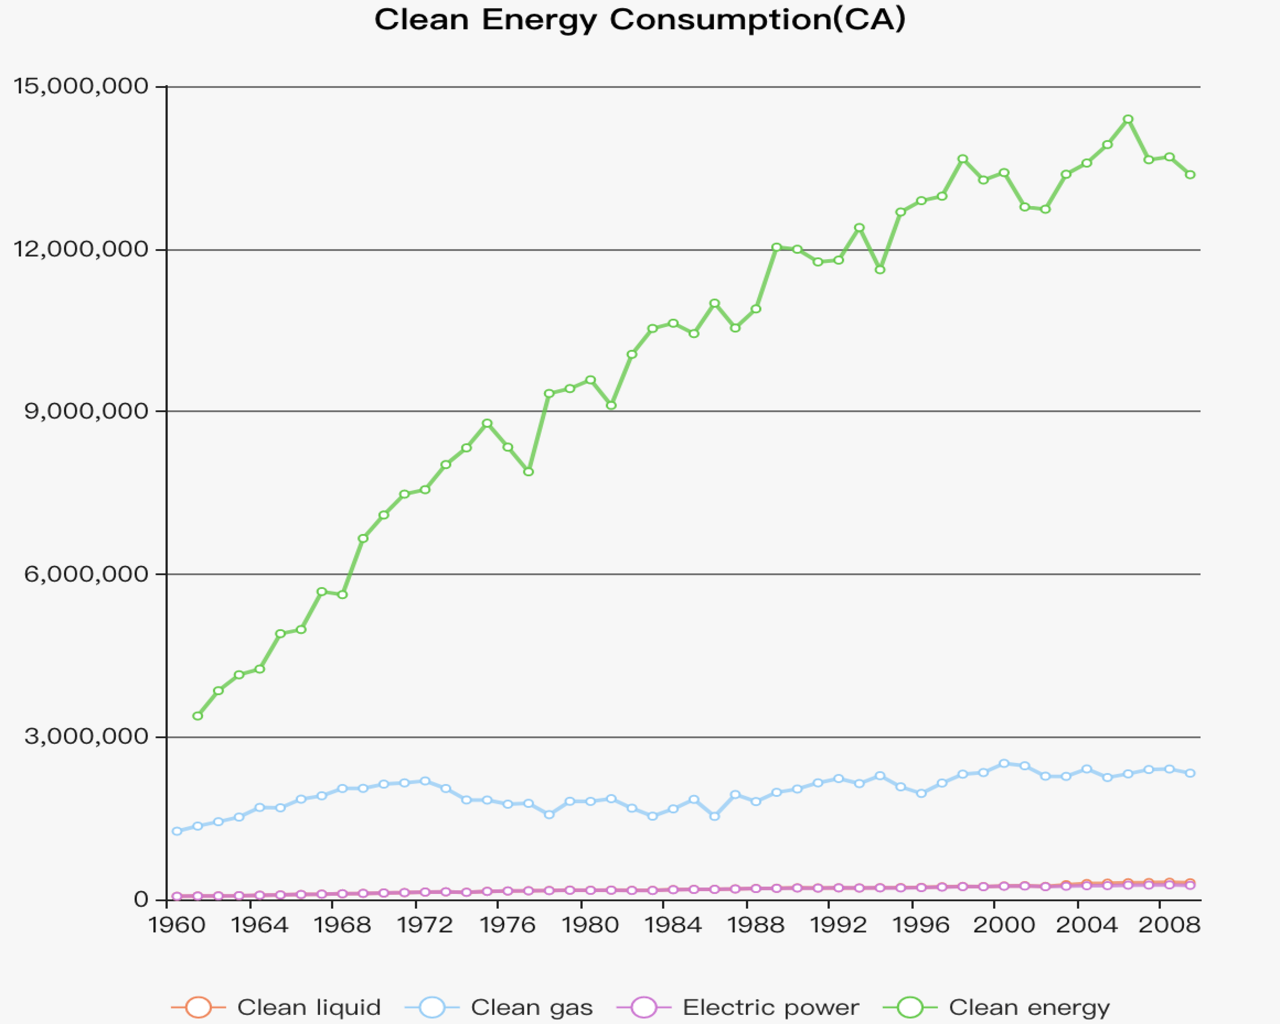
\includegraphics[width=2.2in]{./11_gaitubao_com_1280x1024.png}
\label{fig:side:a}
\end{minipage}%
\begin{minipage}[t]{0.5\linewidth}
\centering
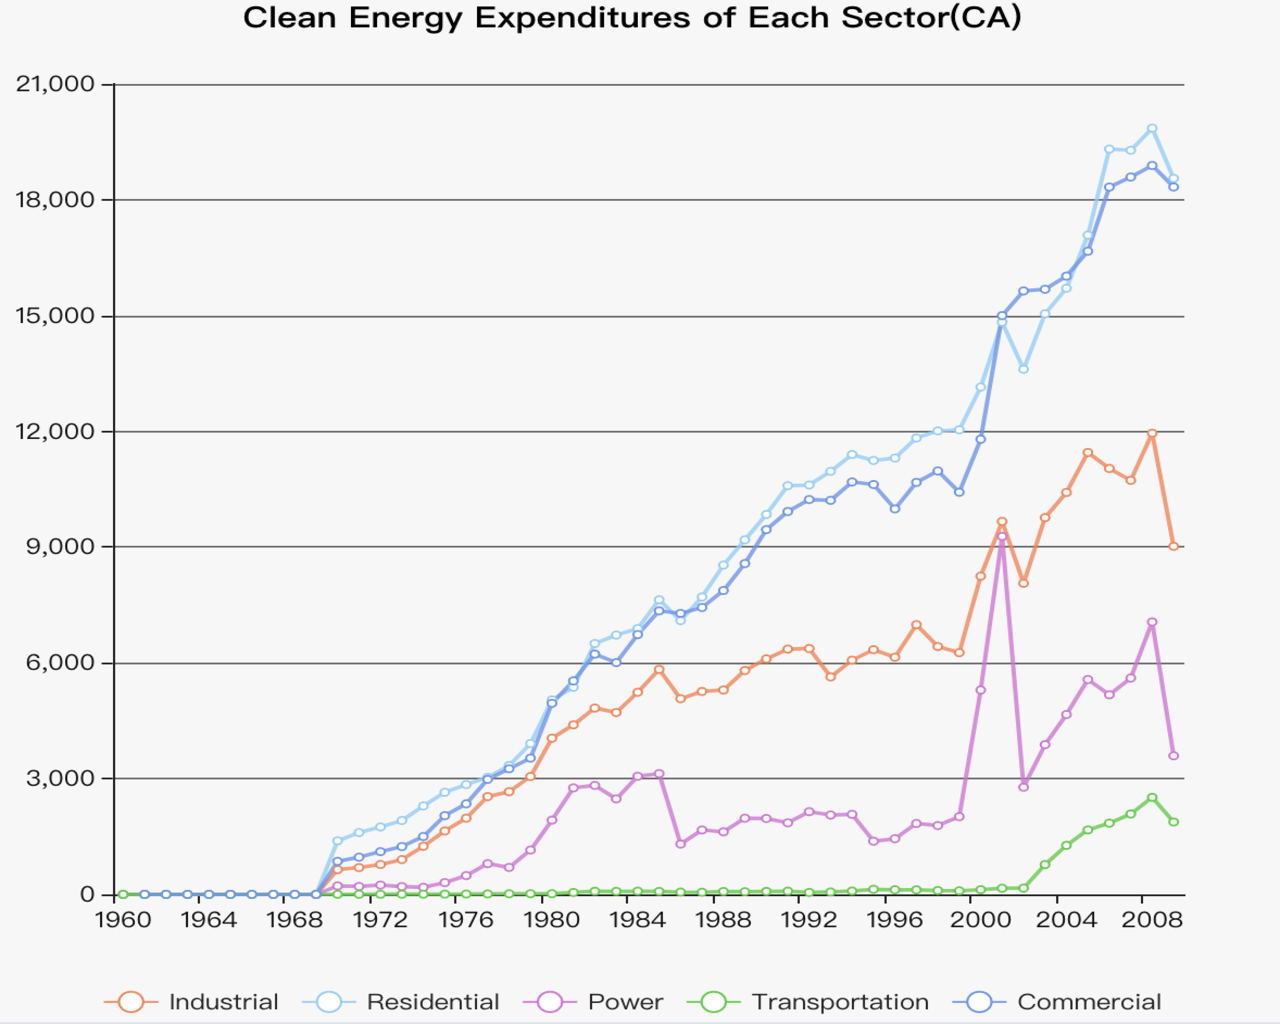
\includegraphics[width=2.2in]{./13_gaitubao_com_1280x1024.png}
\label{fig:side:b}
\end{minipage}
\end{figure}

\begin{figure}[H]
	\begin{center}
		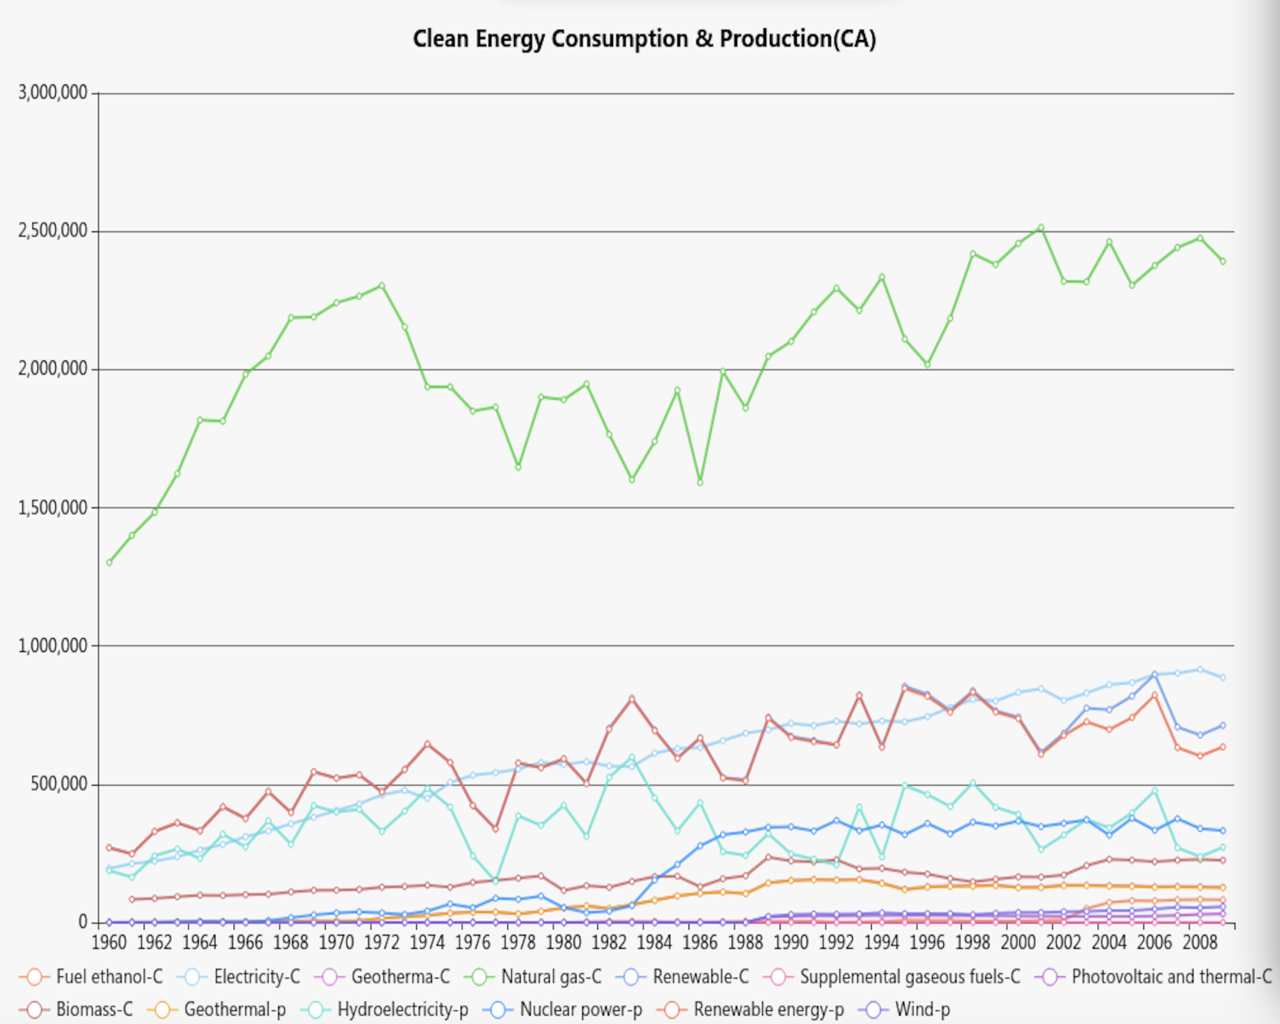
\includegraphics[width=0.5\linewidth]{2018021200475294897CAAA.png}
		\caption{Evolution of clean and reliable energy(CA)}
		\label{Fig:1}
	\end{center}
	\vspace{-0.5em}
\end{figure}


\begin{enumerate}
\item The clean energy consumption in CA state has been fluctuating in the period of 1960~2008. The consumption of natural gas is still generally higher than that of electric power consumption.

\item In terms of the clean energy expenditures in each sectors of CA state,that in residential and commercial sector is the largest. Expenditure in the industrial sector has fluctuated and the electric power sector peaked around 2002, and that in the transportation sector has risen significantly after 2002 years.

\item In terms of clean energy consumption or production of CA state, the consumption of natural gas is far more than that of other clean energy consumption. The electric power consumption is steadily rising, approaching a straight line. It is worth mentioning that the state's renewable energy consumption and the output of renewable energy basically coincide, indicating that renewable energy is less imported and less exported. The energy output of the state is dominated by wind power, and nuclear power is supplemented by nuclear power, and nuclear power is mainly developed around 1981.
\end{enumerate}


\begin{figure}[H]
\begin{minipage}[t]{0.5\linewidth}
\centering
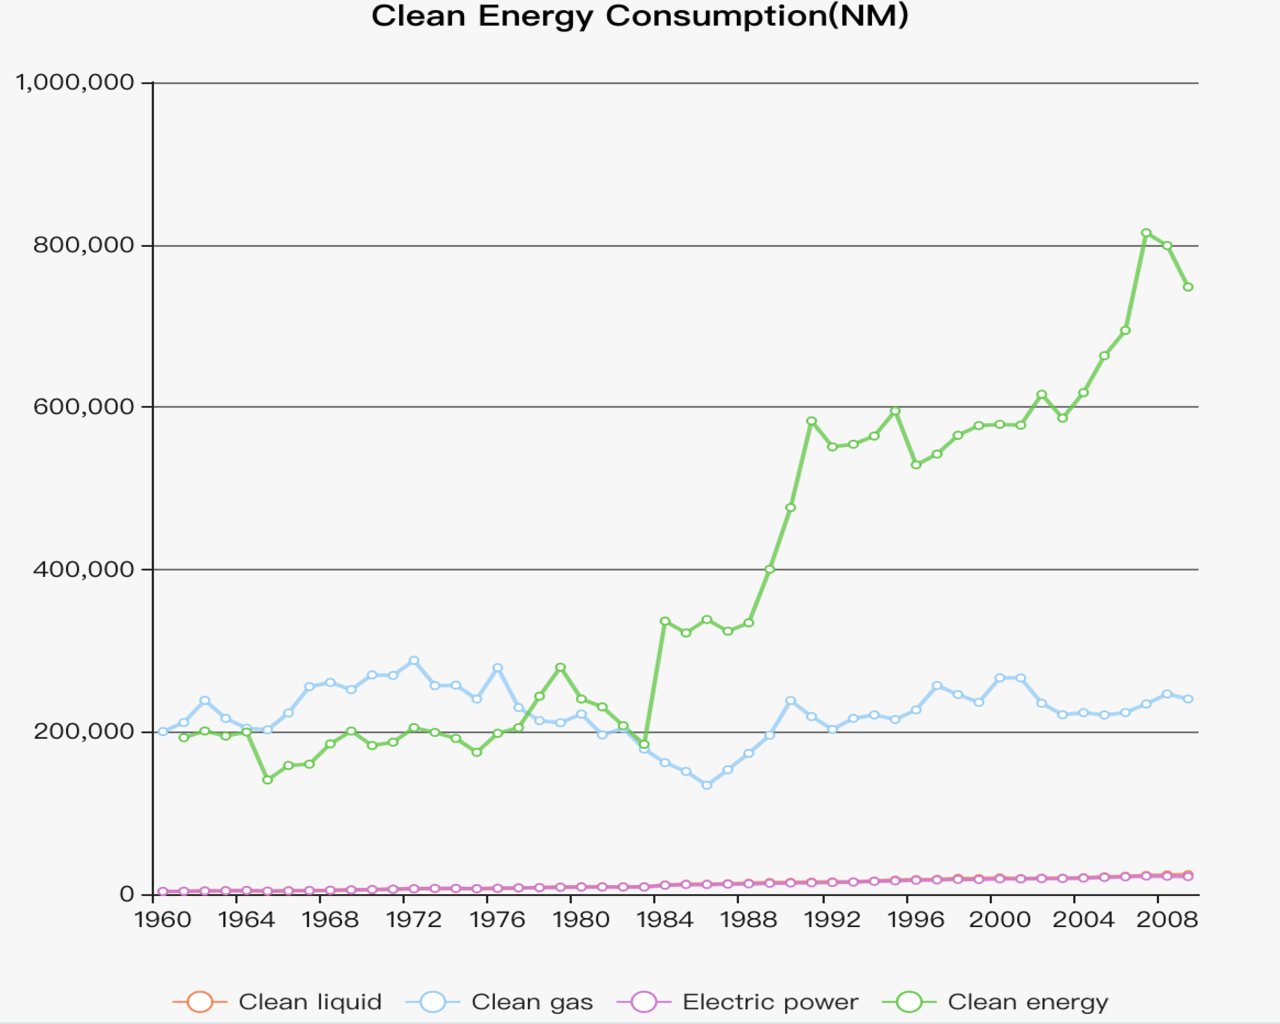
\includegraphics[width=2.2in]{./21_gaitubao_com_1280x1024.png}
\label{fig:side:a}
\end{minipage}%
\begin{minipage}[t]{0.5\linewidth}
\centering
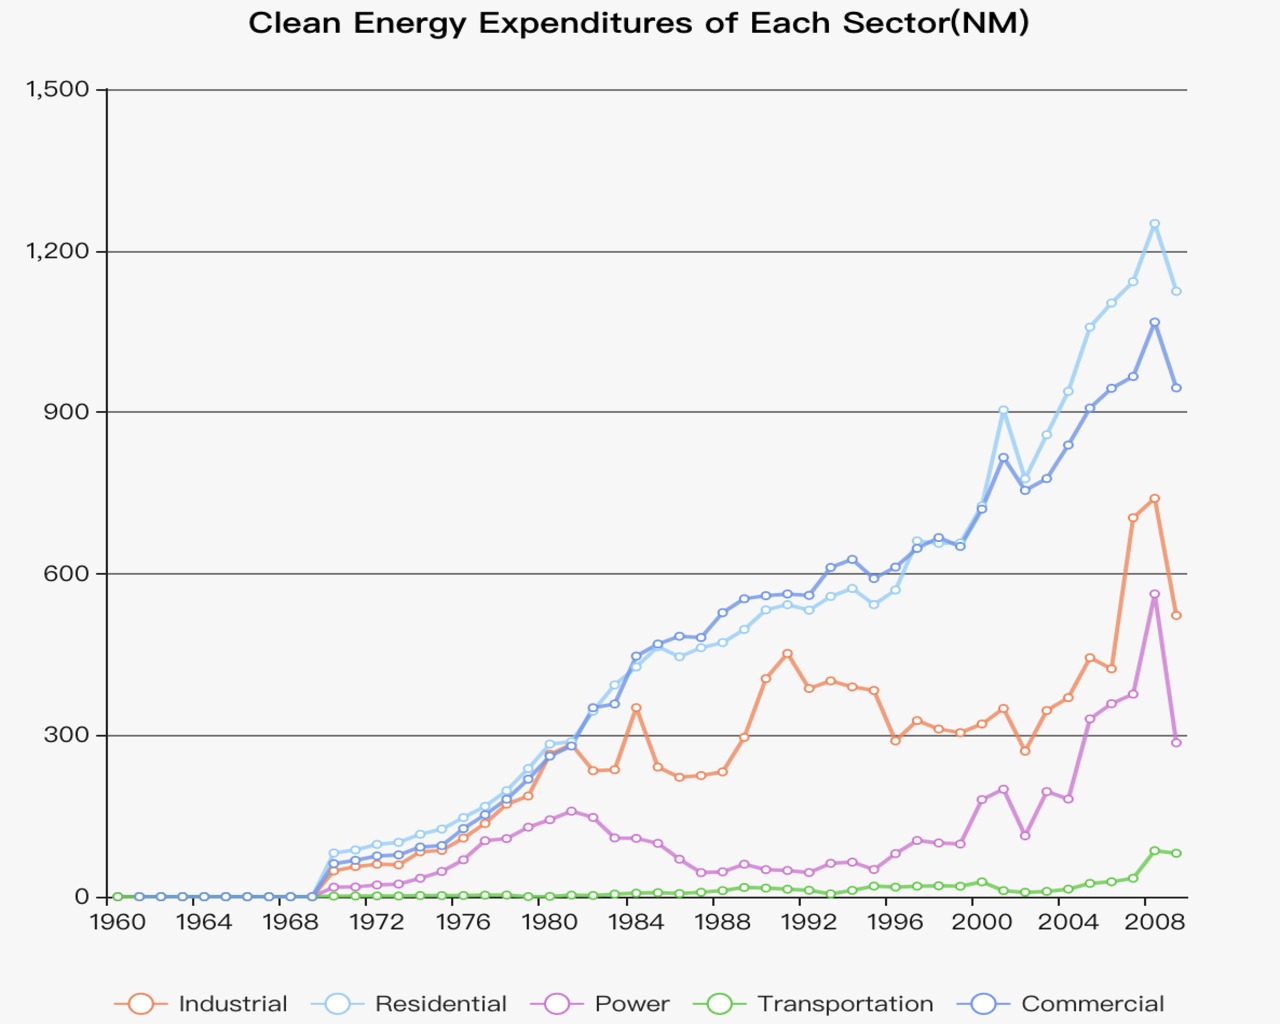
\includegraphics[width=2.2in]{./23_gaitubao_com_1280x1024.png}
\label{fig:side:b}
\end{minipage}
\end{figure}

\begin{figure}[H]
	\begin{center}
		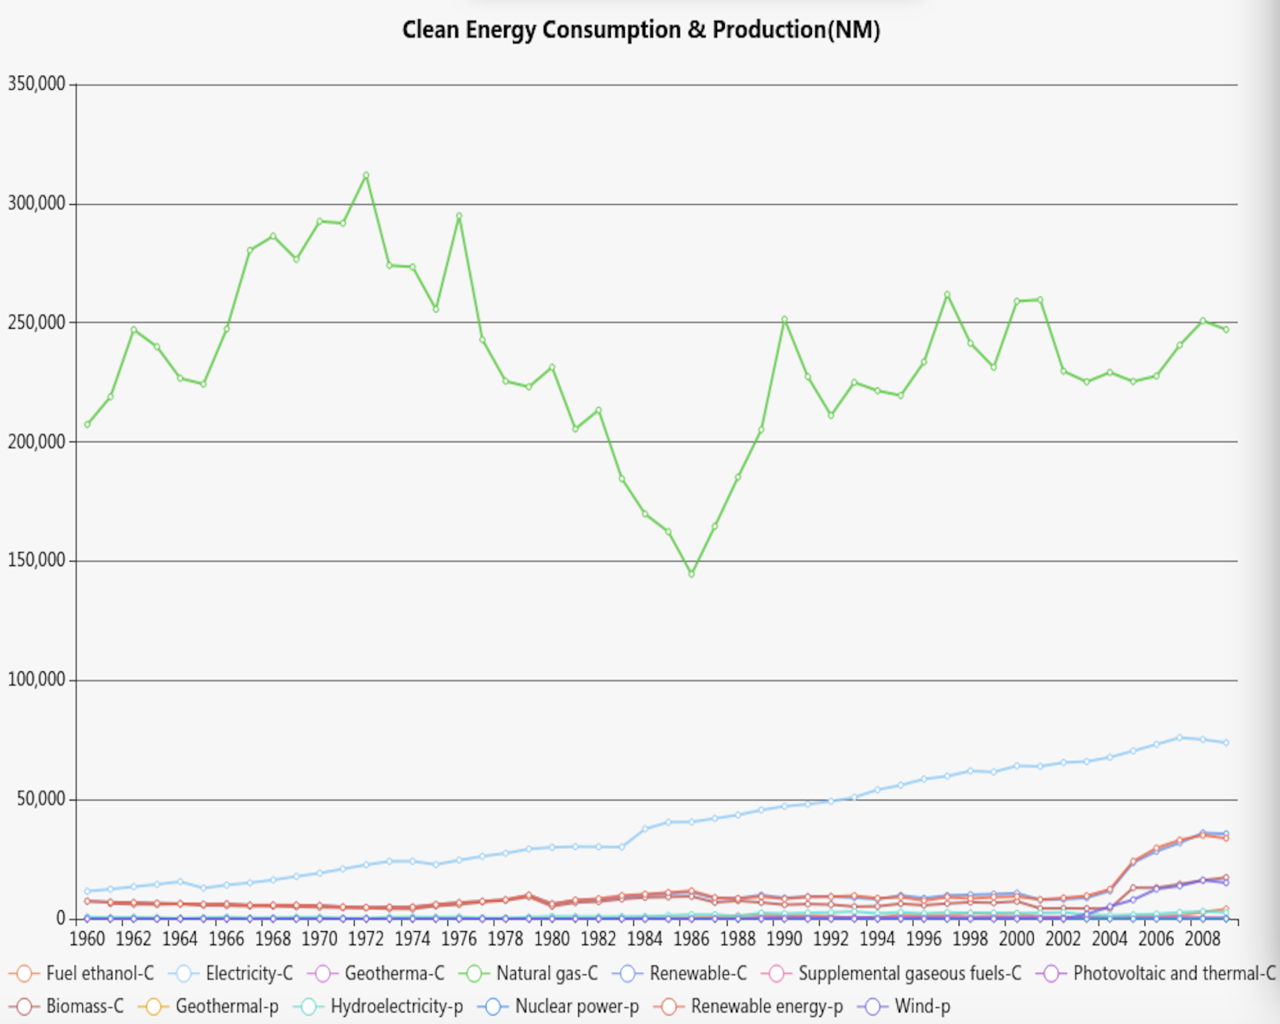
\includegraphics[width=0.5\linewidth]{2018021200482040477NMMM.png}
		\caption{Evolution of clean and reliable energy(NM)}
		\label{Fig:1}
	\end{center}
	\vspace{-0.5em}
\end{figure}

\begin{enumerate}
\item The clean energy consumption in NM states was relatively stable from 1960 to 1978 and rapidly increased after 1978, with an overall upward trend in 1978-2008, reaching a peak around 2007.

\item In terms of the clean energy expenditures in each sectors of NM state, that in the residential sector accounts for relatively low and is less volatile. The expenditure of the electric power sector and the industrial sector is in the middle. The transport sector and the commercial sector are growing, both far exceeding those of other sectors.

\item In terms of clear energy consumption or production of NM state,the largest proportion of natural gas is found, and the consumption of natural gas is much higher than that of other clean energy. There was a large fluctuation from 1960 to 1986, and it increased rapidly from 1987 to 1991.Electric power consumption is steadily rising and less fluctuating. Other energy consumption is not obvious.

\item In terms of energy output, renewable and hydroelectric power were the major outputs. Other outputs were basically in a downtrend before 2004 and showed an upward trend in 2004. Most transportation pollution in NM states followed by industrial pollution, indicating that NM State industrial development, polluted energy accounted for the majority.
\end{enumerate} 

\begin{figure}[H]
\begin{minipage}[t]{0.5\linewidth}
\centering
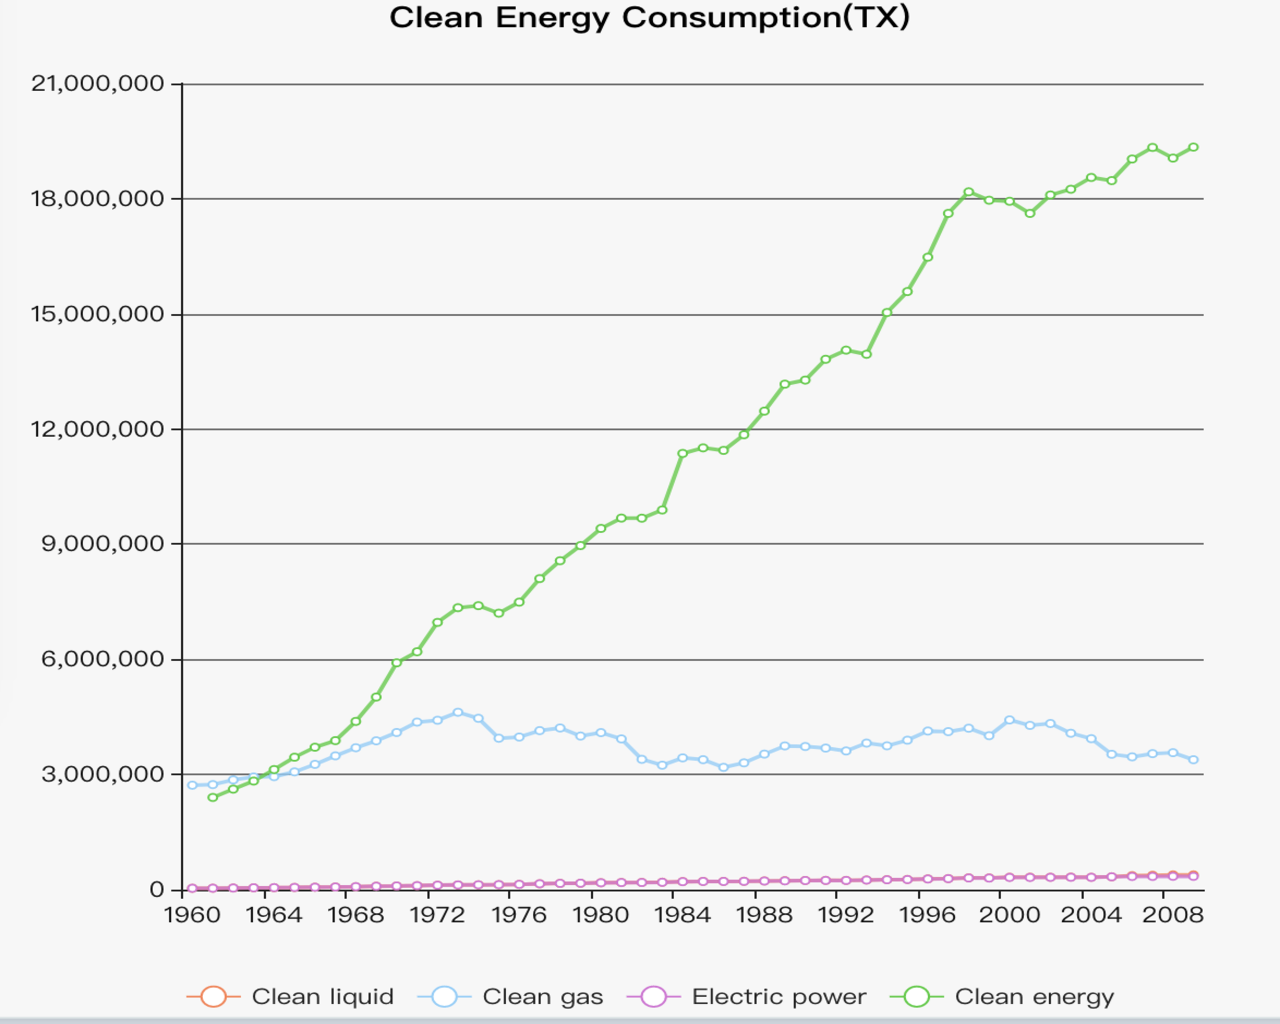
\includegraphics[width=2.2in]{./31_gaitubao_com_1280x1024.png}
\label{fig:side:a}
\end{minipage}%
\begin{minipage}[t]{0.5\linewidth}
\centering
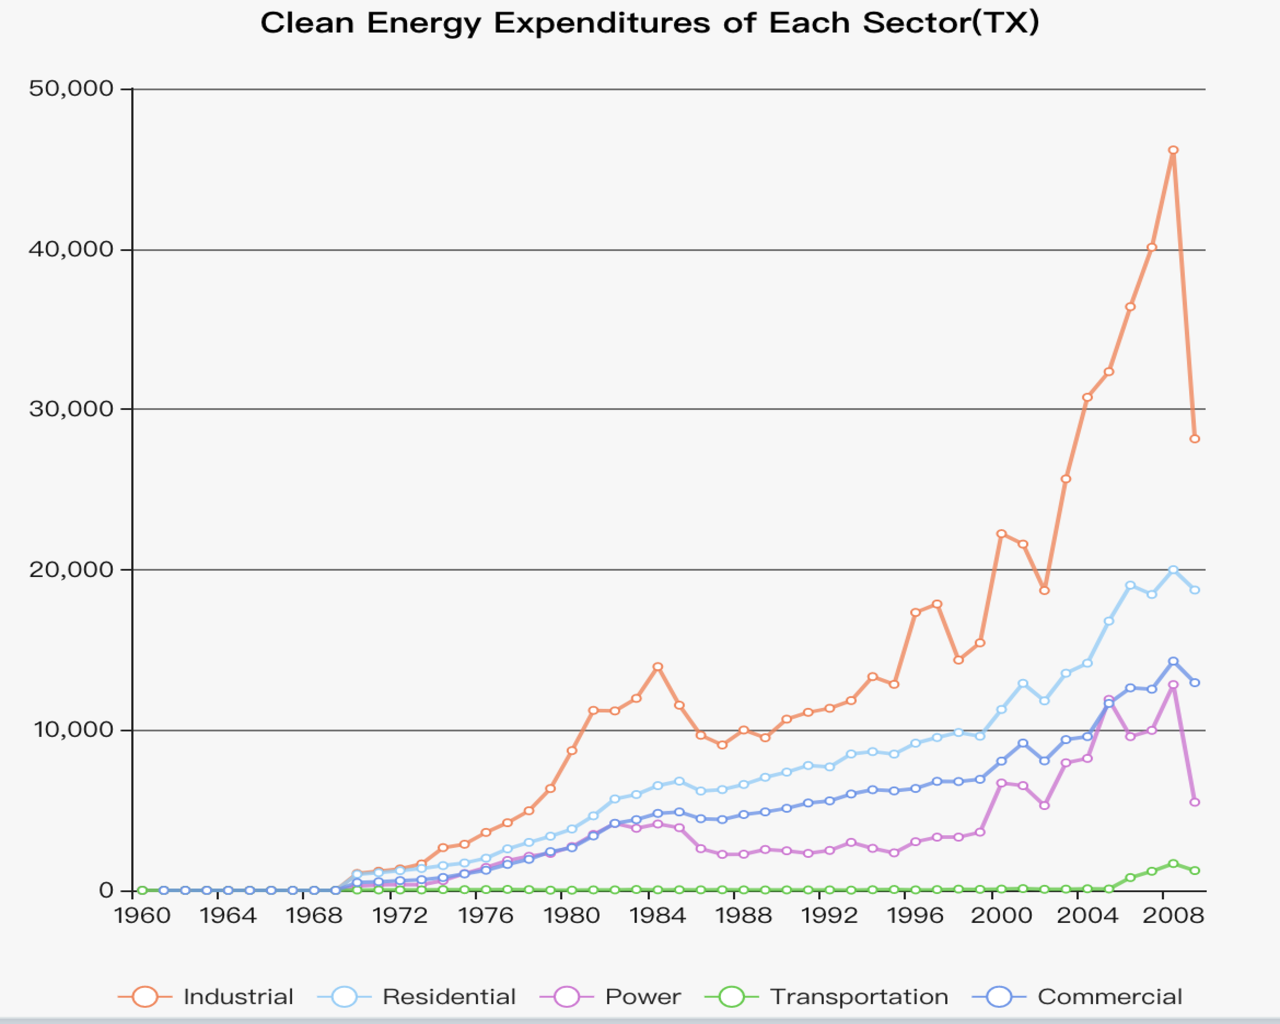
\includegraphics[width=2.2in]{./33_gaitubao_com_1280x1024.png}
\label{fig:side:b}
\end{minipage}
\end{figure}

\begin{figure}[H]
	\begin{center}
		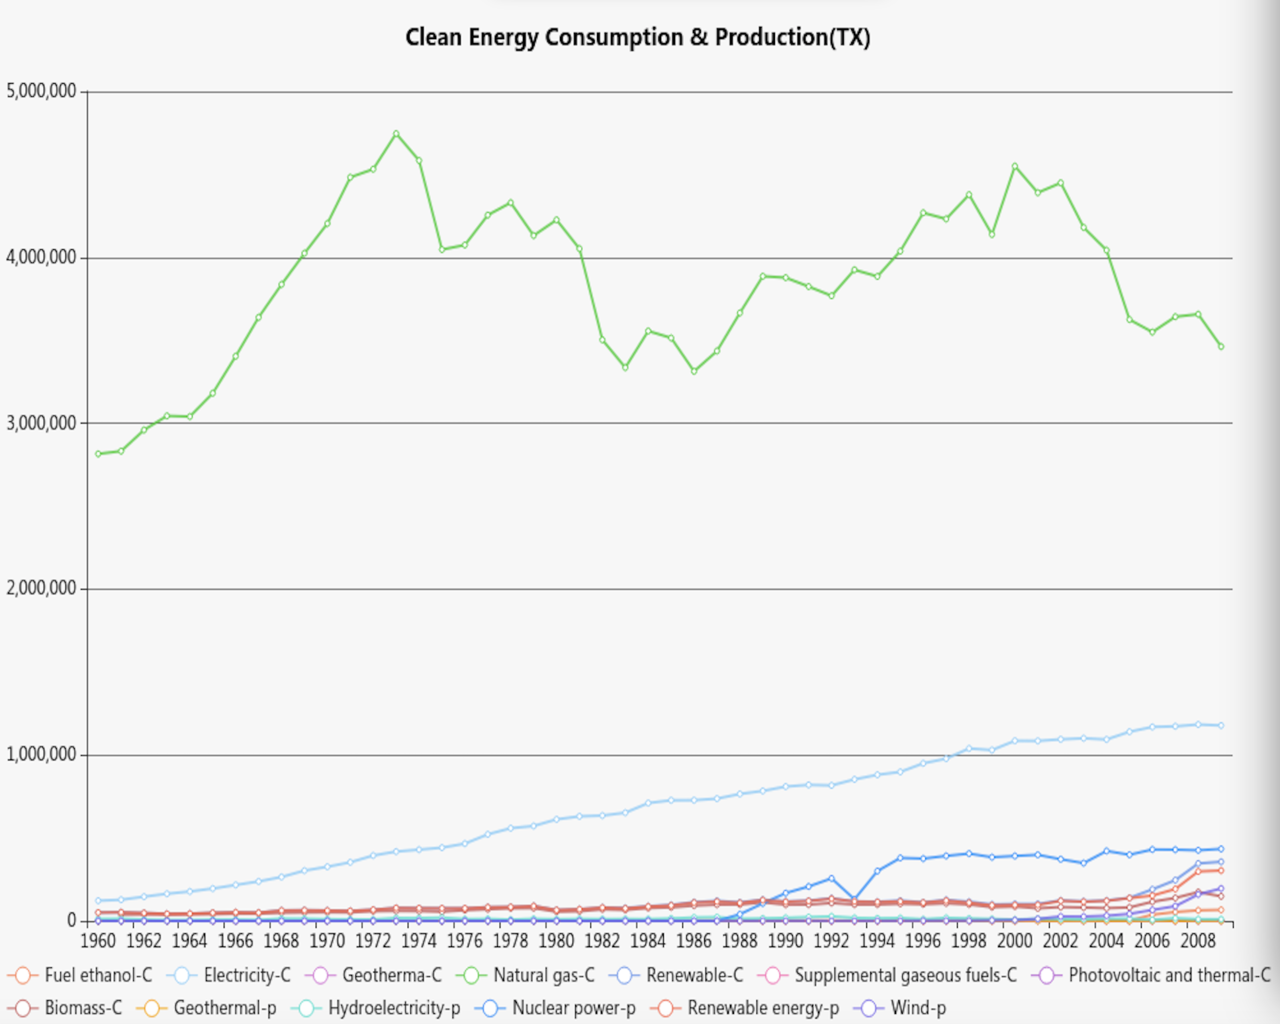
\includegraphics[width=0.5\linewidth]{2018021200484313368TXXX.png}
		\caption{Evolution of clean and reliable energy(TX)}
		\label{Fig:1}
	\end{center}
	\vspace{-0.5em}
\end{figure}

\begin{enumerate}
\item In the clean energy consumption of TX state, the growth of clean energy is fast and almost straight up. On the contrary, the growth of electric power energy is rather slow,which is close to the X axis.And the gas clean energy  is relatively stable. It shows that energy consumption in TX state is more stable, and the speed of clean energy consumption is quicker.

\item In terms of the clear energy expenditures in each sectors of TX state, that in the industrial sector accounted for the largest, followed by the residential sector, the business sector and the power sector, the transport sector is almost zero.It may be related to population and geographical environment of the state, the state is located in the south of heat and air conditioning may  be used too much.

\item In terms of clear energy consumption or production of CA state, the largest proportion of natural gas is found. The consumption of natural gas accounts for the most . There is a large fluctuation between 1960 and 1986 and 1988 to 2008. And Electric power consumption is steadily rising and less fluctuating. Other energy consumption is less.

In terms of energy output, it is worth mentioning that the nuclear power generation began to develop in 1988, very fast, but at the beginning of 1996, the speed was basically stable.

\end{enumerate}

\subsection{Find universal evaluation standard coefficient of usage of clean energy}

After worked out the regulars, we find that they are all much of a muchness. So we can create a model to make a universal evaluation standard of the usage of clean energy.

\subsubsection{Data Expected}

Consolidate all data on 'clean energy consumption', 'clean liquid energy consumption', 'clean gas energy consumption' and 'clean electricity consumption' into a matrix of 50 rows and 4 columns. After topsis processing, a data of 50 Vector t1.

Make all the data about 'the average price of clean energy' into a matrix of 50 rows and 1 column, get a vector t2 of length 50 after topsis processing.

 Put all the information about 'the total expenditure of the commercial sector on clean energy', 'the total expenditure of the industrial sector on clean energy', 'the total expenditure of the electric power sector on clean energy', 'the total expenditure of the residential sector on clean energy', 'The transport sector in the sum of expenditure on clean energy' data to form a matrix of 50 rows and 5 columns, after topsis processing to get a length of 50 vector t3.
 
Make all the data about 'clean energy production' into a matrix of 50 rows and 1 column. After topsis processing, we get a vector t4 of length 50.

If we get the four vectors, and then their average will be the really vector of universal evaluation standard of usage of clean energy. They can be concluded in the following table:

\begin{table}[!htbp]
\centering
\begin{tabular}{cc}
\toprule
Name & Description\\
\midrule
t1 & Clean energy consumption\\
t2 & The average price of clean energy\\
t3 & The total expenditure of each sector on clean energy\\
t4 & Clean energy production\\
\bottomrule
\end{tabular}
\caption{Four vectors}\label{tab:aStrangeTable}
\end{table}

\subsubsection{Topsis method}

In order to find out the really 50 length evaluation coefficient vector, we will find out the four vectors. In order to find out the four vectors, we will evaluate a specific matrix consists of features for each year of each state, finally get a specific number. Then taking into the years, the number will be a 50 length vector.

We decide to use topsis method for every matrix.\cite{topsis} TOPSIS was one of the most famous classics methods first proposed by Hwang and Yoon in 1981 and further expanded by Chen and Hwang in 1992. It introduces two basic concepts: the ideal solution and the negative ideal solution, through the closest ideal solution and the farthest from the negative ideal solution to determine the optimal choice, for the problem has strong applicability and reliability.

For each matrix, the specific calculation steps are as follows:

First of all, we get a 50*n matrix, that is, find the n column features in every year, and make them into a matrix. Then normalize it according to the above explanation (compressing all the data into a small interval to eliminate the dimension). The input is a 50*n matrix, and the output Is a 50-point score that indicates the score of all the columns in each row.

\[r_{ij} = \frac{X_{ij}}{\sqrt[2]{\sum_{k=1}^{4}{X_{kj}^{2}}}},\quad i=1,..,50\quad j = 1,..,n\]

Then, using the algorithm of the maximum difference method, the weight matrix is calculated because the diagonal value of the weight matrix is the weight vector. Because the weight matrix itself has only diagonal values, the others are all 0's. Therefore, the maximum difference method of weight formula is as follows:

\[W_j = \frac{V_j}{\sum_{j=1}^{50}{V_j}}\]

Next, find the ideal solution and the non-ideal solution, that is, the optimal solution and the worst solution:

\[A^{+} = \{v_{1}^{+}, ...v_{n}^{+}\}\]

\[A^{-} = \{v_{1}^{-}, ...v_{n}^{-}\}\]

After that, we calculate the Euclidean distance of each column reaching the optimal solution and the worst solution:

\[D_{i}^{+} = \sqrt[2]{\sum_{j=1}^{n}{v_{ij}-v_{j}^{+}}}, i=1,..,50\]

\[D_{i}^{+} = \sqrt[2]{\sum_{j=1}^{n}{v_{ij}-v_{j}^{-}}}, i=1,..,50\]

Finally, calculate the scores of each line, the end of the entire algorithm:

\[C_i = \frac{D_{i}^{-}}{D_{i}^{+} + D_{i}^{-}}\]

\subsubsection{Get the evaluation coefficient}

According to topsis method\cite{topsis2}, we choose features matrix as Table 3, then we will divided it into 4 parts as 3.3.1. Then we will input these matrix into topsis model to evaluate the four matrix until they all become 50 length vector. Mark them as t1, t2, t3, t4.

So the evaluation coefficient $C_i$(i means 1960-2009) will be:

\[C_i = (t_1 + t_2 + t_3 + t4) / 4\]

$C_i$ can together the four factors: assumption, average price, expenditures of each sector and production.

\subsubsection{Data visualization}

After the topsis method, we got all the evaluation coefficient for each year of each state.

The result is:

\begin{figure}[H]
	\begin{center}
		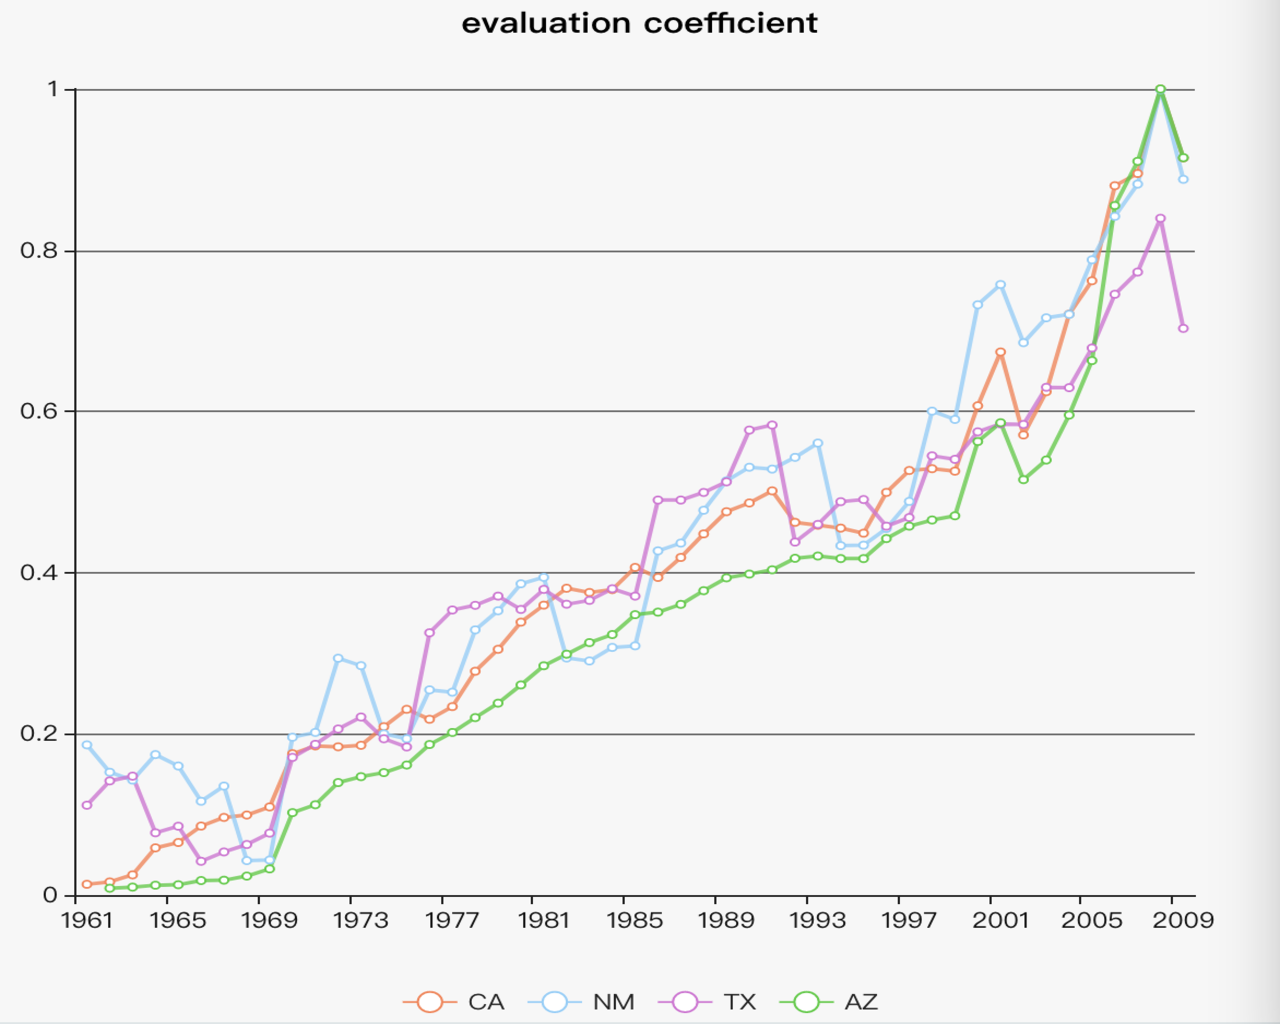
\includegraphics[width=0.5\linewidth]{ec_gaitubao_com_1280x1024.png}
		\caption{Evolution of evaluation coefficient}
		\label{Fig:1}
	\end{center}
	\vspace{-0.5em}
\end{figure}

We found that they have the same trend. Constant growth and fluctuation within a narrow range. To view as a whole, in the past 60 years, TX and NM are better in most time.

What needs to be explained is that the result does not tally with the result of 3.4. It is because we choose different features which we think can be better to describe this time, 21 centuries. 

\subsection{Compare four state in 2009}

Next, we use the topsis method just like 3.3.2 to calculate and compare scores for the four states in the matrix, respectively, for a clean and reliable energy source in which of the four states in 2009 would have the best profile. 

We select 20 features just like 3.1, the method is same. So here we don't list the features. But the number of features are more than 3.3. Because 2009 is near our days, so we need to choose more features to match the size of information. Finally we use topsis to evaluate the 4*20 (4 states, 20 features) matrix, and get a 4 length vector to evaluate the four state.

If you want to get the result in other year, you can execute the three step:

\begin{itemize}
\item 1. Find n specific features, get 4*n matrix.
\item 2. Topsis method to evaluate the matrix.
\item 3. Get the answer.
\end{itemize}

In particular, we only consider the energy-related data of the four states in 2009 and perform reasoning analysis. Data from other years are neglected. The results showed that:

\begin{table}[!htbp]
\centering
\begin{tabular}{cccc}
\toprule
AZ & CA & NM & TX\\
\midrule
0.468 & 0.489 & 0.453 & 0.480\\
\bottomrule
\end{tabular}
\caption{Results}\label{tab:aStrangeTable}
\end{table}

CA> TX> AZ> NM, indicating that AZ State's clean energy profile in 2009 was the best.


\section{Difference analysis}

\subsection{Between state}
% 根据上述的结果发现各个州之间的能源综合指数(evaluation coefficient),四条线之间有什么区别,根据自己对这四个州的地理、人口、行业繁荣度、和其他的因素,给出一个合理的解释出来。
In terms of geography and climate, AZ is in the southwestern part of the United States, and belongs to the subtropical arid and semi-arid climate. The biomass resources based on cotton are very rich. It is suitable for people to live in general. CA is located in the southwestern part of the United States and the east coast of the Pacific. The Mediterranean climate is very pleasant, and the biomass resources are also abundant. 

At the same time, natural gas and oil reserves are also sufficient, which is very suitable for people to live and work.NM is in the west, the climate is dry, it has the most abundant energy and mineral, but also because of the climate reasons, it is not suitable for people to live. TX is in the southwest, temperate or subtropical climate, rich in storage, and is also very suitable for people to live and work.

In terms of the perspective of economic and industrial structure, CA's economy is the most developed in four states, and it has aerospace, electronics, refining, petrochemical and other emerging industries or traditional energy industries. It has the largest manufacturing center in the west, so it is dominated by non clean energy in energy use.The economy of TX state is ranked second in four states. In the early twentieth Century, the discovery of oil led to economic prosperity, and the development of high-tech industry began in 1980s. 

Therefore, TX has more coal and power plants, refineries and processing industries. But in recent years, the consumption of clean energy is accelerating. Especially wind power is ranked first in the United States. And the economy of AZ and NM is relatively backward, so energy consumption is still dominated by non clean energy.

From the perspective of population and state area, CA state has the largest population in four states, but the area size is discharged. This indicates that the employment situation in this state is very good, and the side reaction also may bring more non clean energy consumption, and the industry is in urgent need of transformation. 

In the four states, the state of TX has a population of second and an area of second, with considerable potential for reform of the energy structure. NM state has the least population and an area of second. It should focus on solving the problem of industrial pollution and developing new industries. The area and population of AZ state are third, and AZ is steadily developing. If it is guided by policy, there is a lot of space for steady development.

\subsection{In state}

We decide to use multiple regression analysis to work out this question.\cite{mr1}

The dependent variable is $y$, that is, the energy evaluation index above.The k independent variables affecting the dependent variable are ,$x_1$,...,$x_k$.

We find six features in 605 variables that are unrelated to energy, or variables with severe regional factors, which are:
\begin{itemize}
\item 1. Real gross domestic production
\item 2. Current-dollar gross domestic production
\item 3. Resident population including Armed Forces
\item 4. Biomass total consumption
\item 5. Total energy production
\item 6. Total energy consumption
\end{itemize}

Those features are the independent variables $x_1, x_2, x_3, x_4, x_5, x_6$

It is assumed that the influence of every independent variable on the dependent variable y is linear. That is to say, when the other independent variables remain unchanged, the mean value of y will change uniformly with the change of independent variables.

Suppose , $y=k_0 + k_1 x_1 + k_2 x_2 + k_3 x_3 + k_4 x_4 + k_5 x_5 + k_6 x_6.$ The $k_0,...,k_6$ are the regression parameters, in which $k_1,...,k_6$ indicate the weight of each feature's contribution to the state energy evaluation index, that is, the influence factor.

Model parameters $k_0,...,k_6$ are estimated by using sample data. The model was trained 50 times, and the y' value and y value were compared each time, and the value of $k_0,...,k_6$ was constantly corrected. Finally, the most influential factors of 6 factors in each state were obtained.

It needs to be explained that the reason why we use multivariate linear regression instead of neural network and polynomial regression is that the latter two are relatively heavy fitting. We only need to get weight analysis to construct a single function and do not need to do the fitting analysis.

Final result:

\begin{table}[!htbp]
\centering
\begin{tabular}{cccc}
\toprule
AZ & CA & NM & TX\\
\midrule
-7.570e-07 & 9.111e-08 & 2.013e-06 & 3.515e-07\\
2.5131e-06 & 3.558e-07 & 7.366e-06 & 1.278e-08\\
-4.734e-05 & -1.76e-05 & -2.05e-04 & 1.201e-05\\
7.4863e-06 & 5.570e-07 & 7.463e-06 & 1.375e-06\\
5.6898e-07 & 4.134e-08 & 4.952e-07 & 5.381e-08\\
8.9949e-08 & 3.413e-08 & 1.705e-07 & -3.29e-08\\
\bottomrule
\end{tabular}
\caption{Results}\label{tab:aStrangeTable}
\end{table}

\begin{itemize}
\item AZ:
\end{itemize}

The positive influence factors were Current-dollar gross domestic product, Biomass total consumption, Total energy production and Total energy consumption, of which Current-dollar gross domestic product and Biomass total consumption had a greater impact on the energy evaluation coefficient, indicating that the state's economy is more developed, biomass resources are abundant, and the energy structure is more reasonable. The negative factors are 13, indicating  that in the development of the state, the production and living needs and permanent population factors are still the reasons for the high utilization of clean energy. It may be that the development of industrialization and population or environmental awareness of population have led to the greater utilization of non clean energy.

\begin{itemize}
\item CA:
\end{itemize}

The positive factors were Real gross domestic product,Current-dollar gross domestic product, Biomass total consumption,Total energy production and Total energy consumption, and the impact is more balanced. But if we want to improve the utilization,economy and output of clean energy, these factors need to be enhanced. The negative impact factor is Resident population including Armed Forces, and the weight is large. This indicates that the resident population factor is the main reason to obstruct the utilization of clean energy. It may be that the population is large or the population's environmental awareness is not enough, which leads to the more utilization of non clean energy.

\begin{itemize}
\item NM:
\end{itemize}

The positive factors were Real gross domestic product,Current-dollar gross domestic product, Biomass total consumption,Total energy production and Total energy consumption, of which Real gross domestic product,Current-dollar gross domestic product and Biomass total consumption had a greater impact on the energy evaluation coefficient, indicating that the state's production structure and energy structure were more reasonable, the economy was more developed and biomass resources were abundant. The negative impact factor is 3, indicating that the resident population factor in the state is still the main obstacle to clean energy utilization. It may be that the population is large or the population's environmental awareness is not enough, which leads to the more utilization of the non clean energy.

\begin{itemize}
\item TX:
\end{itemize}

The positive influence factors were Real gross domestic product,Current-dollar gross domestic product,Resident population including Armed Forces,Biomass total consumption and Total energy production, of which Resident population including Armed Forces and Biomass total consumption had a greater impact, This indicates that it is likely to be affected by the policy and that the resident population has a higher awareness of environmental protection.The biomass resources are rich, the energy structure is more reasonable, and the prospects for the development of clean energy are high. The negative impact is 6, indicating that the state is likely to have more energy consumption, thus increasing the consumption of non clean energy.

\section{Predict}

We want to predict the usage of clean energy in 2025 and 2050 according to the data from 1969 to 2009. So we deeply analyzed the data we have, and find that the evaluation coefficient in 3.3 is the best feature to describe the usage of clean energy.

So our task is: according to the evaluation coefficient of 1969-2009, predict the value in 2025 and 2050.

We choose the gray model. With the four states' policies unchanged, the gray model was used to predict the energy status of the four states in 2025 and 2050. Based on the past clean energy features, 50 energy indicators were expanded to 91 Energy indicator data, using the model to amplify the length of 41, resulting in 2025 and 2050 forecast energy value.

Below we will introduce the details:

\subsection{The general form of GM(1, 1)}
Set a variable  $X^{(0)} = \{X^{(0)}(i), i=1,2,..,n\}$ as a non negative monotone raw data column for a predicted object.In order to establish a grey prediction model, first of all,accumulating and generating operators for $X^{(0)}$,then generate an accumulative sequence:

\[X^{(1)} = \{X^{1}(k), k=1,2,3..,n\}\] in which:

\[X^{(1)}(k) = \sum_{i=1}^{k}{X^{(0)}(i)}=X^{(1)}(k-1) + X^{(0)}(k)\]

A differential equation for the following form can be established for $X^{(1)}$:

\[\hat{X}^{(k+1)} = (X^{(0)}[1] - \frac{u}{a})e^{-ak} + \frac{u}{a}\]

or:

\[\hat{X}^{(k+1)} = (X^{(0)}[1] - \frac{u}{a})e^{-a(k-1)} + \frac{u}{a}\]

In the form, K is a time series, which is advisable for year, season, and month.

\subsection{Recognition algorithm}

The sequence of the parameters is $\hat{a} = [a,u]^{T}$,and $\hat{a}$ can be solved by the next formula:

\[\hat{a} = (B^{T}B)^{-1}B^{T}Y_{n}\]

In the format: $B$ is a data matrix, and $Y_n$ is a data column.
\[
B = 
\begin{bmatrix}
-\frac{1}{2}(X^{(1)}(1)+X^{(1)}(2)) \\
\cdots \\
-\frac{1}{2}(X^{(1)}(1)+X^{(1)}(n))

\end{bmatrix}
\]

\[
Y_n = (X^{(0)}(2), X^{(0)}(3), .., X^{(0)}(n))^{T}
\]

\subsection{Reduction of predicted values}
Since the GM model is the cumulative amount of one quantity and is the predictive value of the $k \in{n+1, n+2, ...}$ time, the data $\frac{\hat{X}^{(1)}(k+1)}{\hat{X}^{(1)}(k)}$ of the GM model must be inverse generated and reduced to $\frac{\hat{X}^{(1)}(k+1)}{\hat{X}^{(1)}(k)}$.

\[\hat{X}^{(1)}(1) = \sum_{i=1}^{k}{\hat{X}^{(0)}(1)} = \sum_{i=1}^{k-1}{\hat{X}^{i} + \hat{X}^{(0)}(i)}\]

\[\hat{X}^{(0)}(k) = \hat{X}^{(1)}(k) - \sum_{i=1}^{k-1}{\hat{X}^{(0)}(i)}\]

Because of $\hat{X}^{(0)}(k-1) = \sum_{i=1}^{k-1}(\hat{X}^{(0)}(i))$, so $\hat{X}^{(0)}(k) = \hat{X}^{(1)}(k) - \hat{X}^{(1)}(k-1)$

\subsection{Test one: posterior difference test}

The average value and variance of the actual data of the original data column are as follows:

\[\bar{X} = \frac{1}{n}\sum_{k=1}^{n}{\hat{X}^{(0)}(k)}\qquad S_{1}^{2} = \frac{1}{n}\sum_{k=1}^{n}({X^{(0)}(k) - \bar{X}})^{2}\]

The residual of item k: $q(k) = X^{(0)}(k) - \hat{X}^{(0)}(k)$

The mean and variance of the residuals of all data items in the whole data column are as follows:

\[\bar{q} = \frac{1}{n} \sum_{k=1}^{n}{q(k)} \qquad S_{2}^{2} = \frac{1}{n} \sum_{k=1}^{n}(q(k) - \bar{q})^{2}\]

Posterior difference ratio: $C = \frac{S_2}{S_1}$

The smaller the $C$ is, the closer the estimated value of the grey model is to the actual value.

\subsection{Small error probability}

\[P = P(|q(k) - \bar{q}| < 0.6745S_1\]
The bigger, the better.

\begin{table}[!htbp]
\centering
\begin{tabular}{ccc}
\toprule
Precision grade & Small error probability & Posterior difference ratio\\
\midrule
Good & >0.95 & <0.35 \\
Qualified & >0.8 & <0.5\\
Grudgingly qualified & >0.7 & <0.65\\
Unqualified & 0.65 & <0.7\\
\bottomrule
\end{tabular}
\caption{Posterior difference test and small error probability accuracy grade Table
}\label{tab:aStrangeTable}
\end{table}

\subsection{Result}

The procedure for using gray model for data prediction is shown below:

Step1: Enter a series of 50 length

Step2:  the model for a variety of processing

Step3:  output the sequence of 91 lengths, the posterior difference ratio of the two evaluation accuracy values, and the small probability error of the model on the prediction result. 

The results are shown in the table below, the first and second column of data represents the model test out the value of 2025 and 2050, the third column of data represents the ratio of posterior difference, The fourth row of data represents the small error probability of the 2050 forecast data tested by the model.

\begin{table}[!htbp]
\centering
\begin{tabular}{ccccc}
\toprule
 &2025 &2050 &C & P\\
\midrule
AZ&2.369 &8.441 & 0.079 & 0.98 \\
CA&1.998 &5.845 & 0.059 & 1\\
NM&1.795 & 4.817 & 0.069 & 1\\
TX&1.458 & 3.412 & 0.120 & 0.96\\
\bottomrule
\end{tabular}
\caption{Results}\label{tab:aStrangeTable}
\end{table}

Then, the forecast of the 2025 energy index and the 2050 energy index of the four states obtained by the model are tested, and after the residual test, it is found that:

For all the predicted values $|\epsilon (k)|< 0.1$|, the predicted value reaches a higher requirement.  At the same time, it shows that the prediction accuracy reaches the first accuracy of the gray model, that is, the highest precision.

After that, the states of the clean energy use of each state were plotted, abscissa indicates the year, the time period: 1960-2009, 2025, 2050, ordinate that the use of clean energy.

\begin{figure}[H]
	\begin{center}
		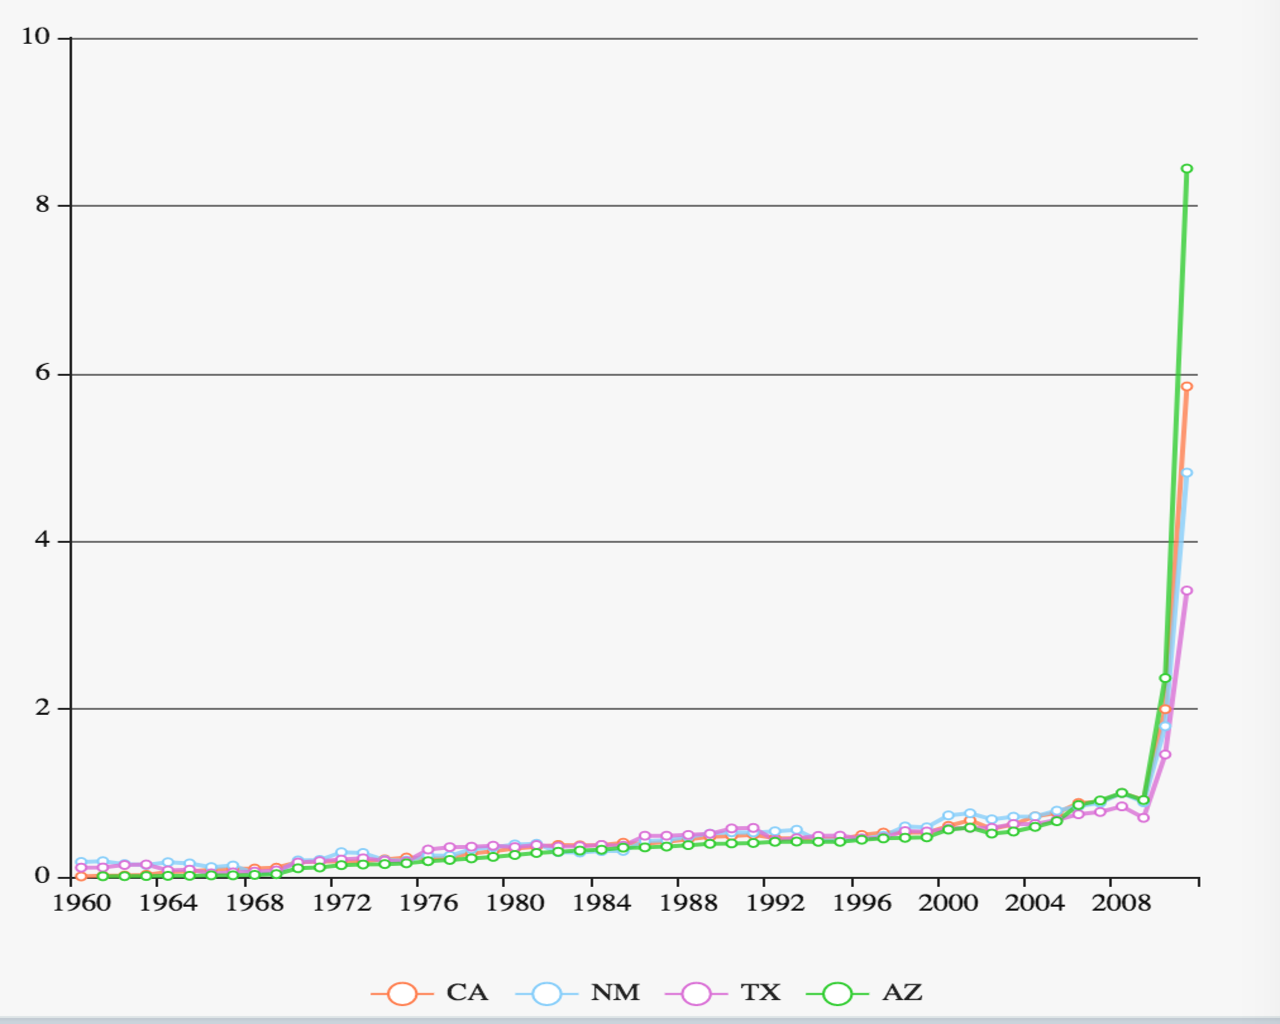
\includegraphics[width=0.5\linewidth]{After_prediction_gaitubao_com_1280x1024.png}
		\caption{Evolution of evaluation coefficient after prediction}
		\label{Fig:1}
	\end{center}
	\vspace{-0.5em}
\end{figure}



\section{Interstate compact}
\subsection{Target}

We forecast the clean energy evaluation coefficient in four states in 2025 and 2050, and we finally conclude that in the absence of any policy change in the governors' office, by 2025, the ranking of clean energy usage in the four states is AZ>CA>NM>TX, while in 2050, the clean energy index ranking in these four states is still AZ>CA>NM>TX.It is predicted that AZ is better in the usage of clean energy in the future, and TZ's usage of clean energy is more severe in the future.

What we need to say is that we define the standard of the best clean energy as large clean energy consumption ,low average price of clean energy , large expenditure of clean energy and high output of clean energy . Based on the similarities and differences between the four states, we set up some future goals for energy development for them\cite{energy}:

\begin{itemize}

\item \textbf{Security:} In order to cope with increasing demand and ensure the supply of energy resources in all States, it is necessary to increase energy production, to expand energy supply and as a result, to increase output.

\item \textbf{Diversification:} To diversify energy sources, diversify sources of energy and diversify energy supply.To exploit alternative clean energy, such as solar energy, wind energy, gas layer, geothermal, biomass energy and so on.

\item \textbf{Modernization:} Through transformation, to realize the modernization of energy infrastructure, so as to ensure the smooth flow of energy transport channels.

\item \textbf{Environmental protection:} To strengthen and improve the energy and ecological environment.

\item \textbf{conservation:} Promote energy conservation and improve energy efficiency in order to prevent the waste and excessive consumption of energy .For example, to promote automobile energy saving and low carbon economy.

\item \textbf{Technology:} To vigorously develop and lead clean energy technologies, to promote timeliness, decisive and effective transformation of energy system, so as to promote the reduction of the average price of clean energy.

\item \textbf{Industry and cooperation:} To promote the transformation of the energy industry. The interstate achieves an energy cooperation mechanism through the integration of energy, environment and economic policies 

\item \textbf{conservation:} promote energy conservation and improve energy efficiency in order to prevent the waste and excessive consumption of energy .For example, to promote automobile energy saving and low carbon economy.

\item \textbf{Technology:} To vigorously develop and lead clean energy technologies, to promote timeliness, decisive and effective transformation of energy system, so as to promote the reduction of the average price of clean energy.

\item \textbf{Industry and cooperation:} To promote the transformation of the energy industry. The interstate achieves an energy cooperation mechanism through the integration of energy, environment and economic policies.

\end{itemize}

\subsection{Six actions}
We think the four local governments in the region can plan their policies and carry out the actions in the following six areas:
\begin{enumerate}
\item Do energy planning, improve the scientific and practical evaluation methods, establish and implement different energy planning systems in different states, encourage the development of high-quality energy sources, and fully consider the potential environmental impacts caused by energy activities.
\item The establishment of a review panel composed of multidisciplinary experts to establish different expert groups for different types of resources planning, sign a cooperation and win-win energy sharing agreement, establish a scientific energy management and evaluation criteria, and be monitored and controlled by a group of experts.
\item Strengthen organization and management, raise civic awareness, establish and improve the system of citizen participation, and issue written documents to fundamentally eliminate energy waste and improve resource utilization.
\item To solve the problem of resource constraints, improve the unreasonable energy structure, increase the proportion of clean energy, improve energy efficiency, improve the supply capacity of the states and improve the level of energy technology and equipment and energy management.
\item To change the mode of extensive economic growth, complement each other's energy to solve the uneven distribution of energy resources in the four states, implement a sustainable energy development strategy, ensure a stable and sustainable interstate energy supply and maintain a reasonable interstate energy The price ensures that the energy needs of the states are met.

\item Save energy, promote the multi-development of energy, strengthen the research and development of energy saving technology and promote the comprehensive utilization of energy.

Actively advocate cooperation in the areas of clean coal technology and efficient utilization of fossil fuels, promote and strengthen cooperation in renewable energy and hydrogen, nuclear energy and other major energy technologies, and discuss the establishment of clean, economic, safe and reliable interstate energy supply system.
\end{enumerate}


\section{Strengths and weakness}
\subsection{Strengths}

The model constructed in this paper has five advantages: high accuracy of model, diversification of model, high matching of model and data, strong innovation of model and practicality of model.

\begin{enumerate}
\item Accuracy:. This model fully considers all the data given by the subject, processes the data effectively, after eliminating the redundant and less relevant data, defines the meaning of the data and extracts the data completely and accurately. Therefore, the model is with high accuracy.

\item Model diversity. This article is to conduct in-depth and comprehensive research on the problem and adopt many different kinds of analysis methods, including TOPSIS tools, PCA analysis methods, multiple regression models and gray prediction models.

\item Matching degree. Due to the extremely high degree of matching between the model and all kinds of data, a more suitable analysis method is selected according to different types of data. Therefore, the results obtained after data input and output have high credibility.

\item Innovation. In this paper, there is a certain uniqueness in model building. When analyzing the energy profiles of the four states, we first use TOPSIS to reduce the dimensionality of the data and then analyze the difference. Secondly, we use the gray model to predict the future energy value Is also a major innovation, not only high precision and can also test correction.

\item Applicability (practicality). This model aims at the practical problems such as uneven energy distribution and large development differences in the four states, determines the energy development goals of the four states in the future, and puts forward the measures that can be taken to achieve the goal. It is practical to solve the energy development problem .

\end{enumerate}

\subsection{Weakness}

It should be noted that, although our data analysis is more complete and comprehensive, but the original data itself has a variety of problems, to our analysis has brought great difficulties and obstacles. Although we use various methods to analyze the data construction model, there are still some shortcomings and deficiencies in our analysis and model. Mainly includes the following three aspects:


\begin{enumerate}
\item  Due to the fact that the data itself is too large and unstable, redundant data is too much, too much data cross, the significance of the data is not obvious and other factors, noise defects, neural networks and other analysis methods will lead to the error is too large, so we deal with the data Simple classification of traditional statistical analysis.

\item Due to the fact that the data type is too large, there is a certain degree of subjectivity inevitable in the human screening data, and the error caused by the data filtering is quite large. Therefore, the model will have some errors. If the data-oriented features are selected for breakthrough, More accurate data, then the accuracy of the model will be further improved.


\item In the analysis of difference, due to the fact that the objective conditions of several intercontinental countries, this paper does not use the numerical model to solve the problem. In addition, when analyzing energy profiles of the four states in 2009, there may be some problems with using previous years data, which may be more accurate when using updated data and model accuracy.

\end{enumerate}


\bibliographystyle{ieeetr}
\bibliography{sample,consumption,topsis,topsis2,mr1,energy}

\newpage
\section{Memo}

\begin{center}
  \textbf{Memo to the governor}
\end{center}

To: Governors 

From: Team \# 73777

Subject: Summary of our paper

Date: Feb.11, 2018

We are glad to hear that your four state governments are seeking a wide range of opinions in order to make reasonable provisions on interstate energy contracts. With the continuous development of the United States in the 21st century, the impact of energy use and production on economic development has become increasingly evident. Only when states sign agreements to cooperate and develop and manage energy technologies can the four states jointly prosper and prosper together.

Although we have not conducted a thorough study of this issue in our model for interstate energy development, we believe some of our core outcomes provide some insights into the development of interstate energy contracts and the development of energy targets for future growth as well as the necessary actions to be taken to achieve that goal.

Firstly, we outline the energy status of the four states in 2009. After entering the data into the model, the following result is obtained, with the highest profile for clean energy in CA (California), followed by TX (Texas), followed by AZ (Arizona), NM (New Mexico State) Clean energy has the lowest profile value.

Secondly, we predict the future energy of the states. The results show that the energy forecast of AZ (Arizona) in 2025 is 2.369, the forecast is much higher than that of other states. The forecast of TX in Texas (TX) is 1.458 in 2025 with a forecast of four The lowest in the state. As for the 2050 energy forecast, the state of AZ still ranks first with a predicted energy value of 8.441. The forecast values of CA (California) and NM (New Mexico) are closer, the forecast of TX is the lowest, and the energy The predicted value is 3.412.

Finally, based on the status quo and the results of the projections, our proposed energy goal is to propose a four-state weighted average of clean energy as a target for energy contracts in order for renewables to reach the same status as all four state.

We hope governors will find this report and help you and your colleagues when you face a win-win energy interstate contract. We wish you the best in your endeavors.

Respectfully.
\end{document}